\section{Problem Set 3}

\subsection{We are Close in Near-Circular Orbits}

\subsubsection{Initial Conditions}
For this problem, we set the initial conditions in classical orbital elements to be [6780000, 0.001, 0, 0, 0, 0]. This provides us with a near circular orbit that is sufficiently far from the attractor's center.

\subsubsection{Initial Conditions in ECI and RTN}
Inertial position and velocity of chief: [6773200, 0, 0, 0, 7700, 0]\\
RTN position and velocity of deputy: [0, 10, 0, 1, 0, 0]

\subsubsection{Integration Constants}

Using the HCW equations, we can find the integration constants based on these initial conditions: [0.0013, 0.0001, -0.0013, -0.0003, 0, 0]

\subsubsection{Propogation with HCW Equations}

\begin{figure}[H]
    \centering
    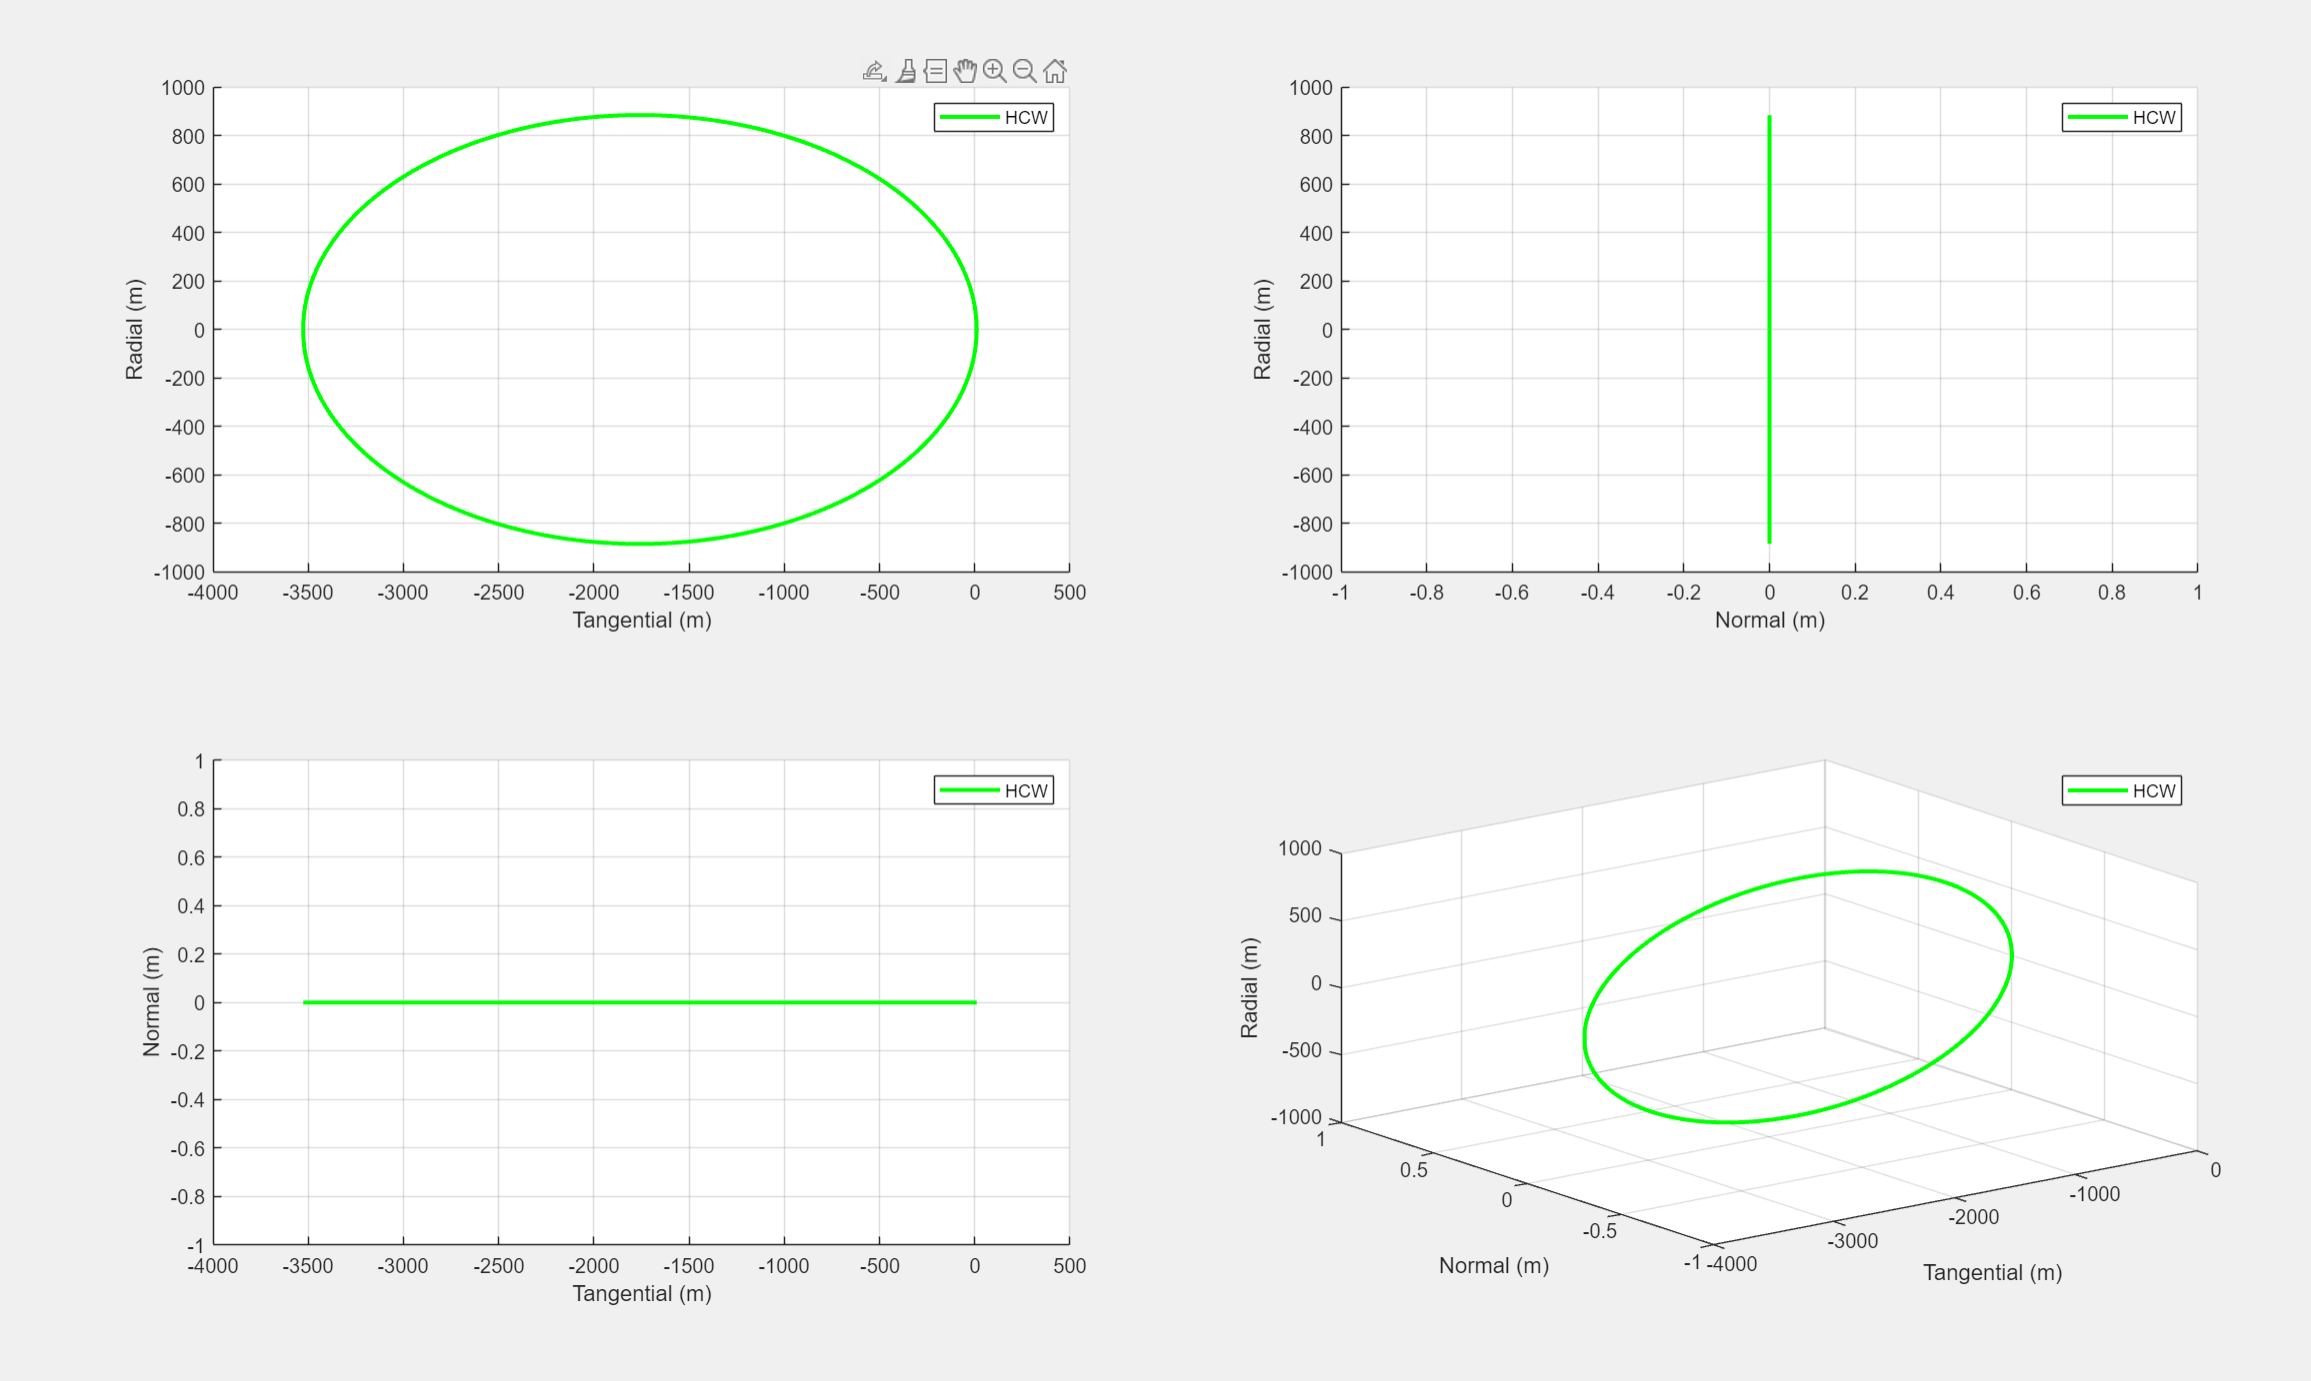
\includegraphics[width=0.7\textwidth]{PS3/Figures/HCW_Position.png}
    \caption{Deputy trajectory in RTN frame from HCW Equations}
    \label{fig:hcw_position}
\end{figure}

\begin{figure}[H]
    \centering
    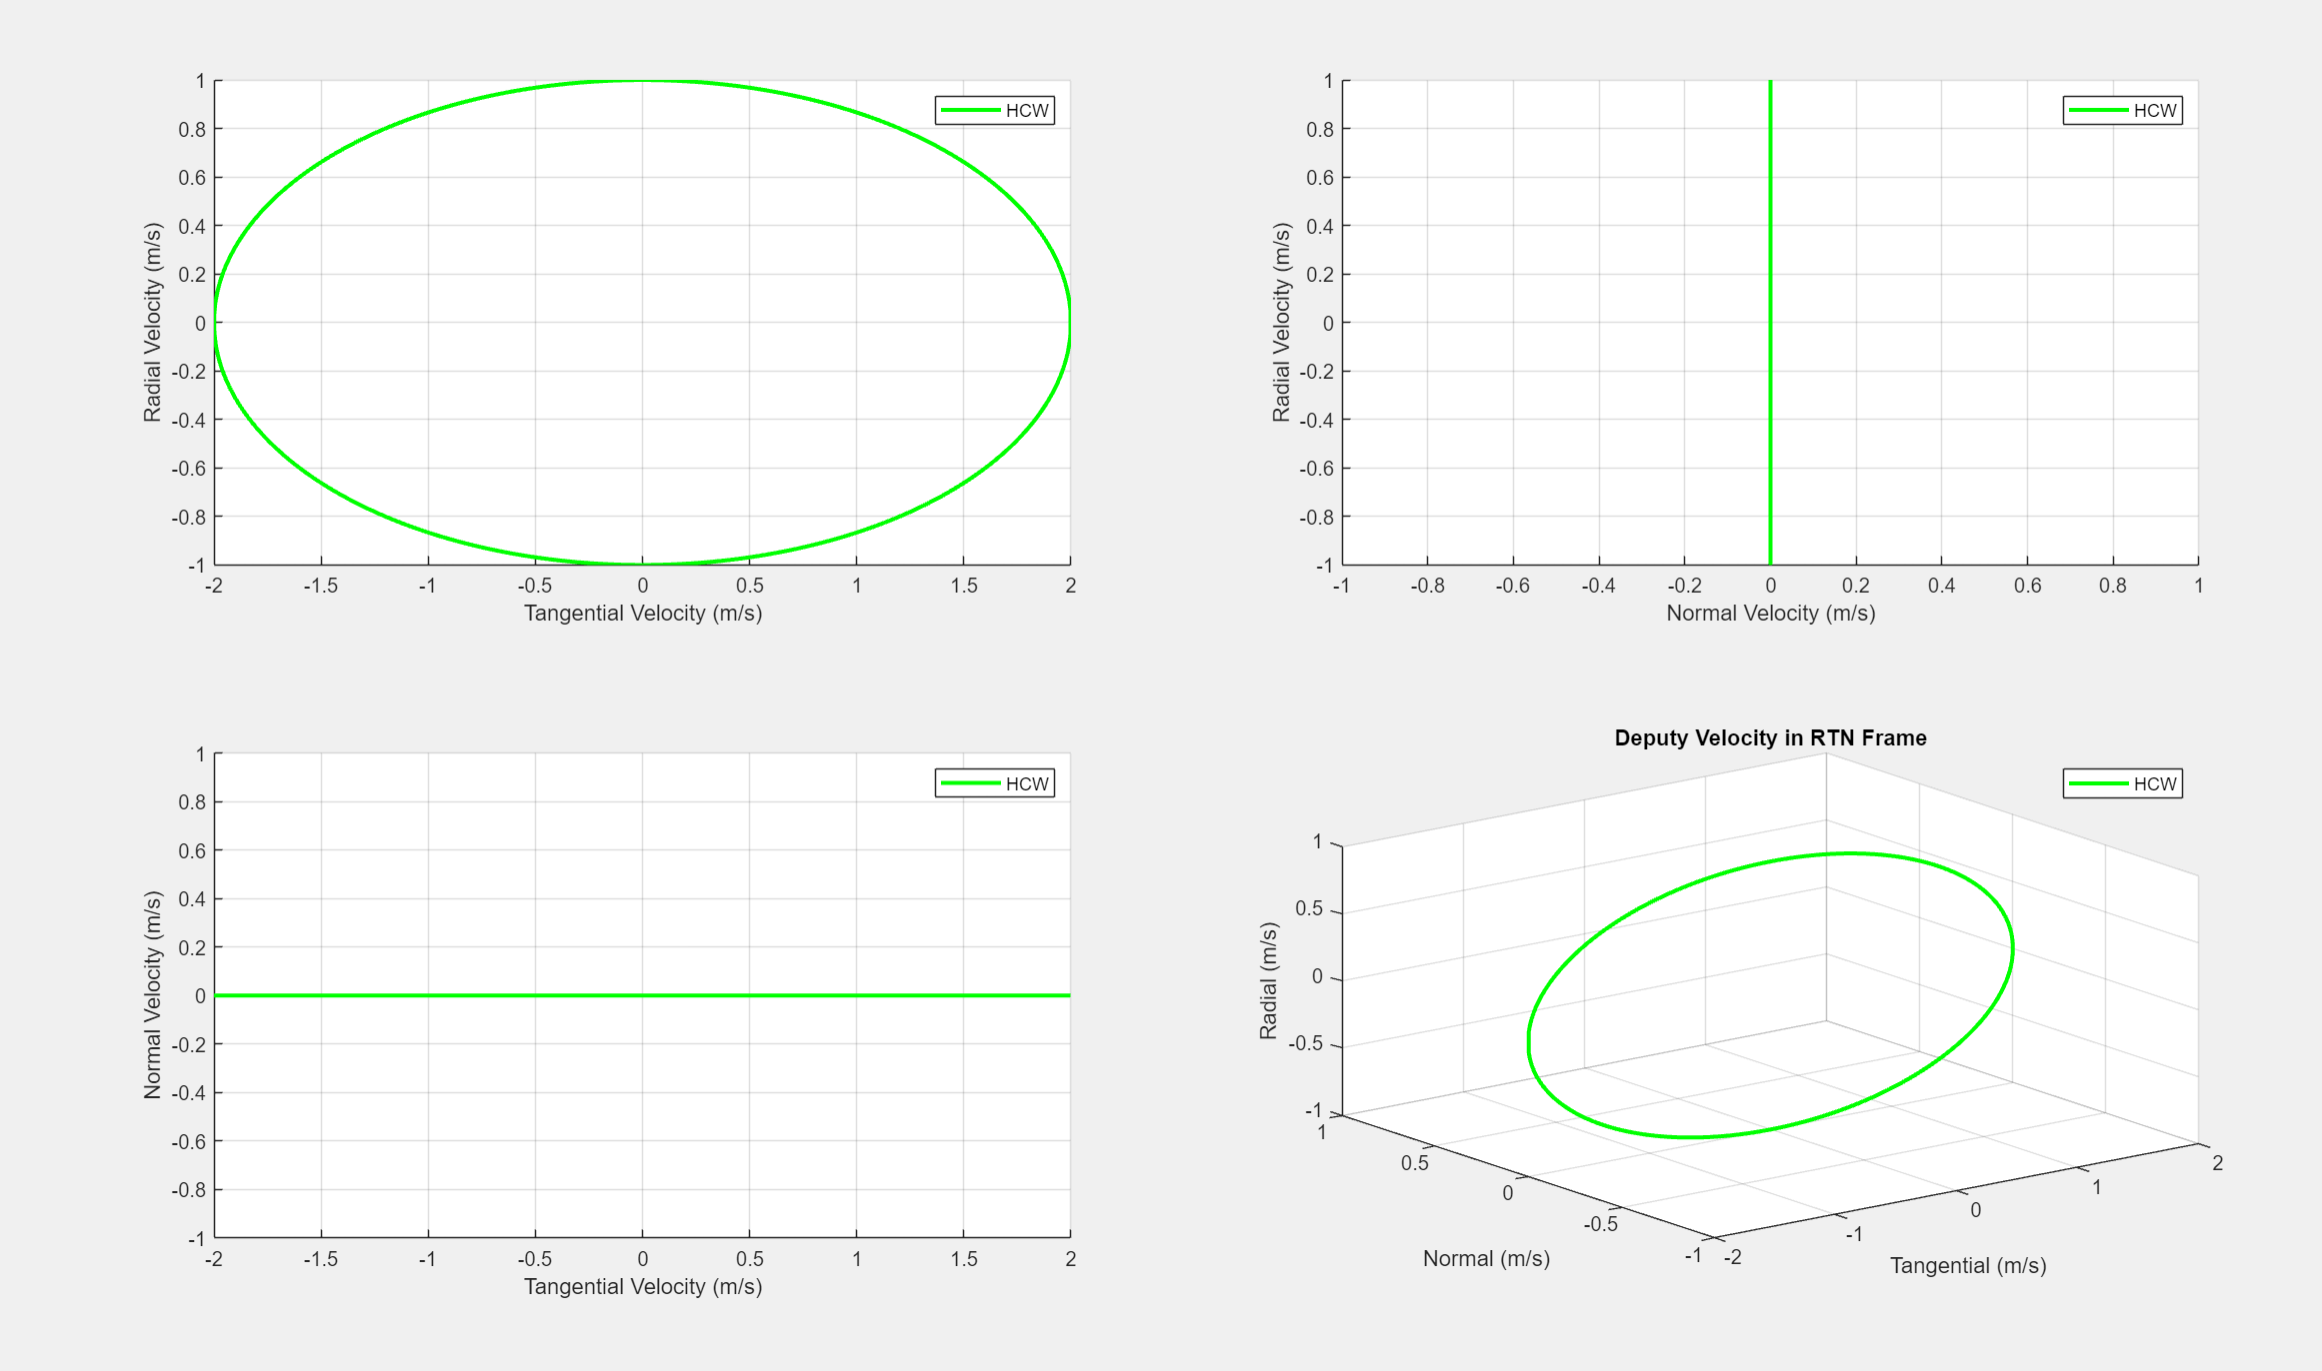
\includegraphics[width=0.7\textwidth]{PS3/Figures/HCW_Velocity.png}
    \caption{Deputy velocity in RTN frame from HCW Equations}
    \label{fig:hcw_velocity}
\end{figure}

\subsubsection{Expected Behavior}

The behavior we see in these plots aligns with expectations. Since the initial conditions involve a difference in the along track direction, with a radial velocity difference, there is no semi major axis difference, and therefore no energy difference, between the orbits. Thus, as expected, we see bounded relative motion with no drift.

\subsection{We are Close in Eccentric Orbits}

\subsubsection{Initial Conditions}
For this problem, we set the initial conditions of the chief in classical orbital elements to be [6780000, 0.1, 0, 0, 0, 0]. This provides us with an eccentric orbit that is sufficiently far from the attractor's center.\\

We set the initial conditions of the deputy to be [0, 10, 0, 1, 0, 0] in RTN as we did for the above problem. This again will give us bounded motion due to the equal energies of the deputy and chief.

\subsubsection{Integration Constants}
We find the integration constants to be: [0, 0.0001072, 0, -0.0002236, 0, 0]

\subsubsection{Propogation with YA Equations}

\begin{figure}[H]
    \centering
    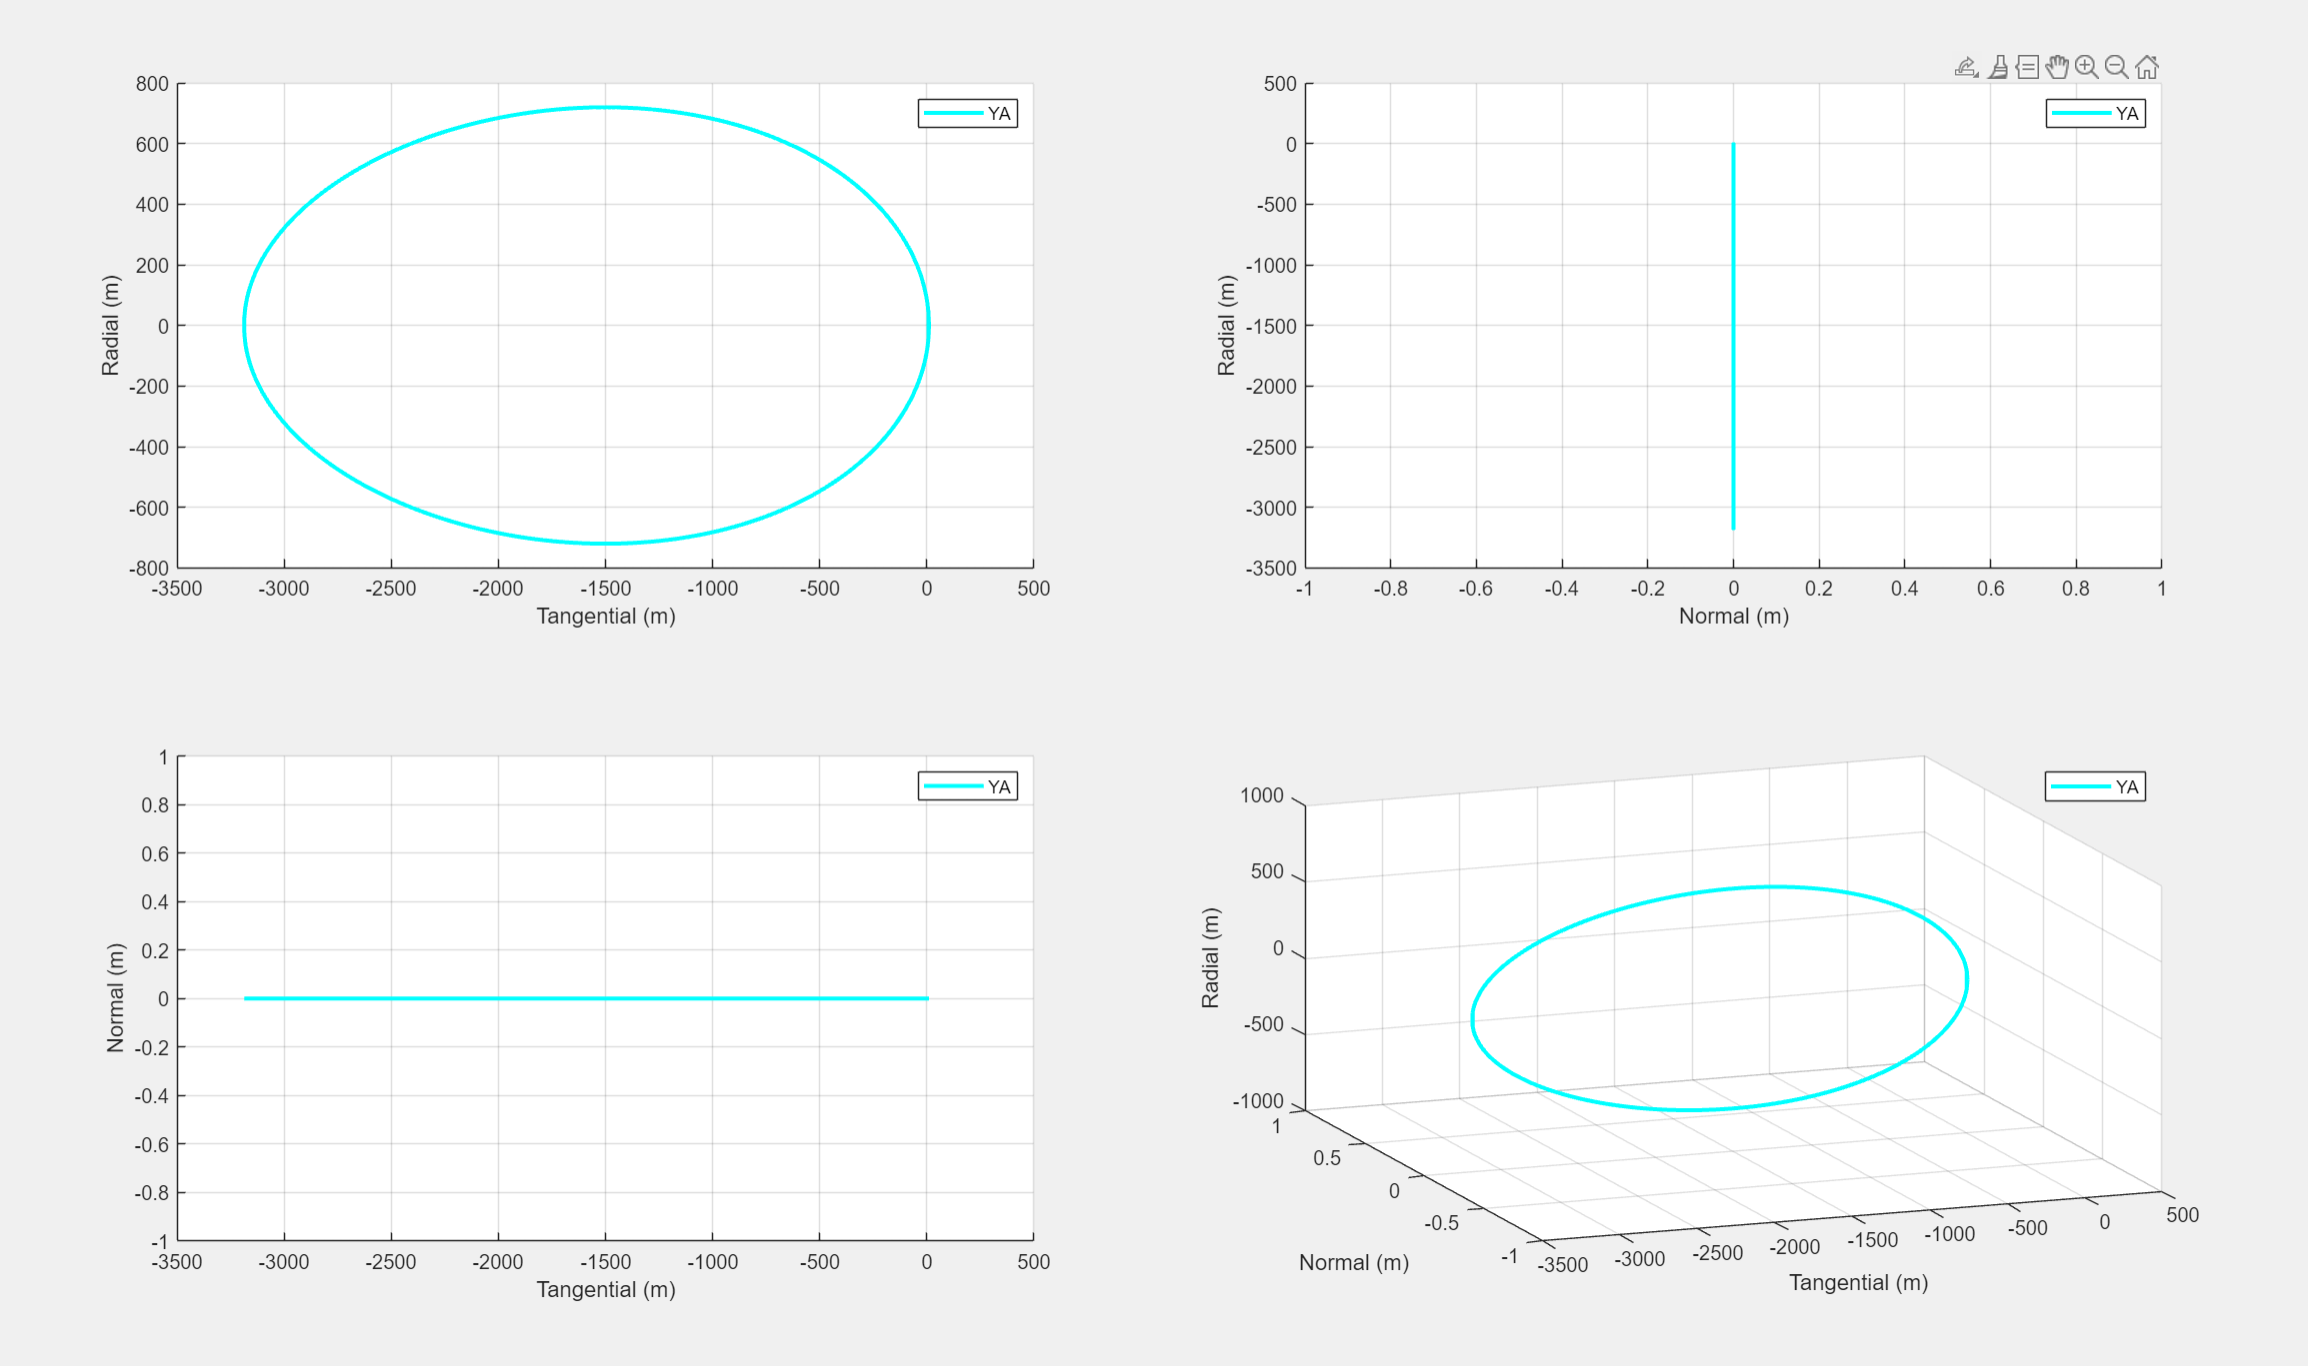
\includegraphics[width=0.7\textwidth]{PS3/Figures/YA_position.png}
    \caption{Deputy trajectory in RTN frame from YA Equations}
    \label{fig:ya_position}
\end{figure}

\begin{figure}[H]
    \centering
    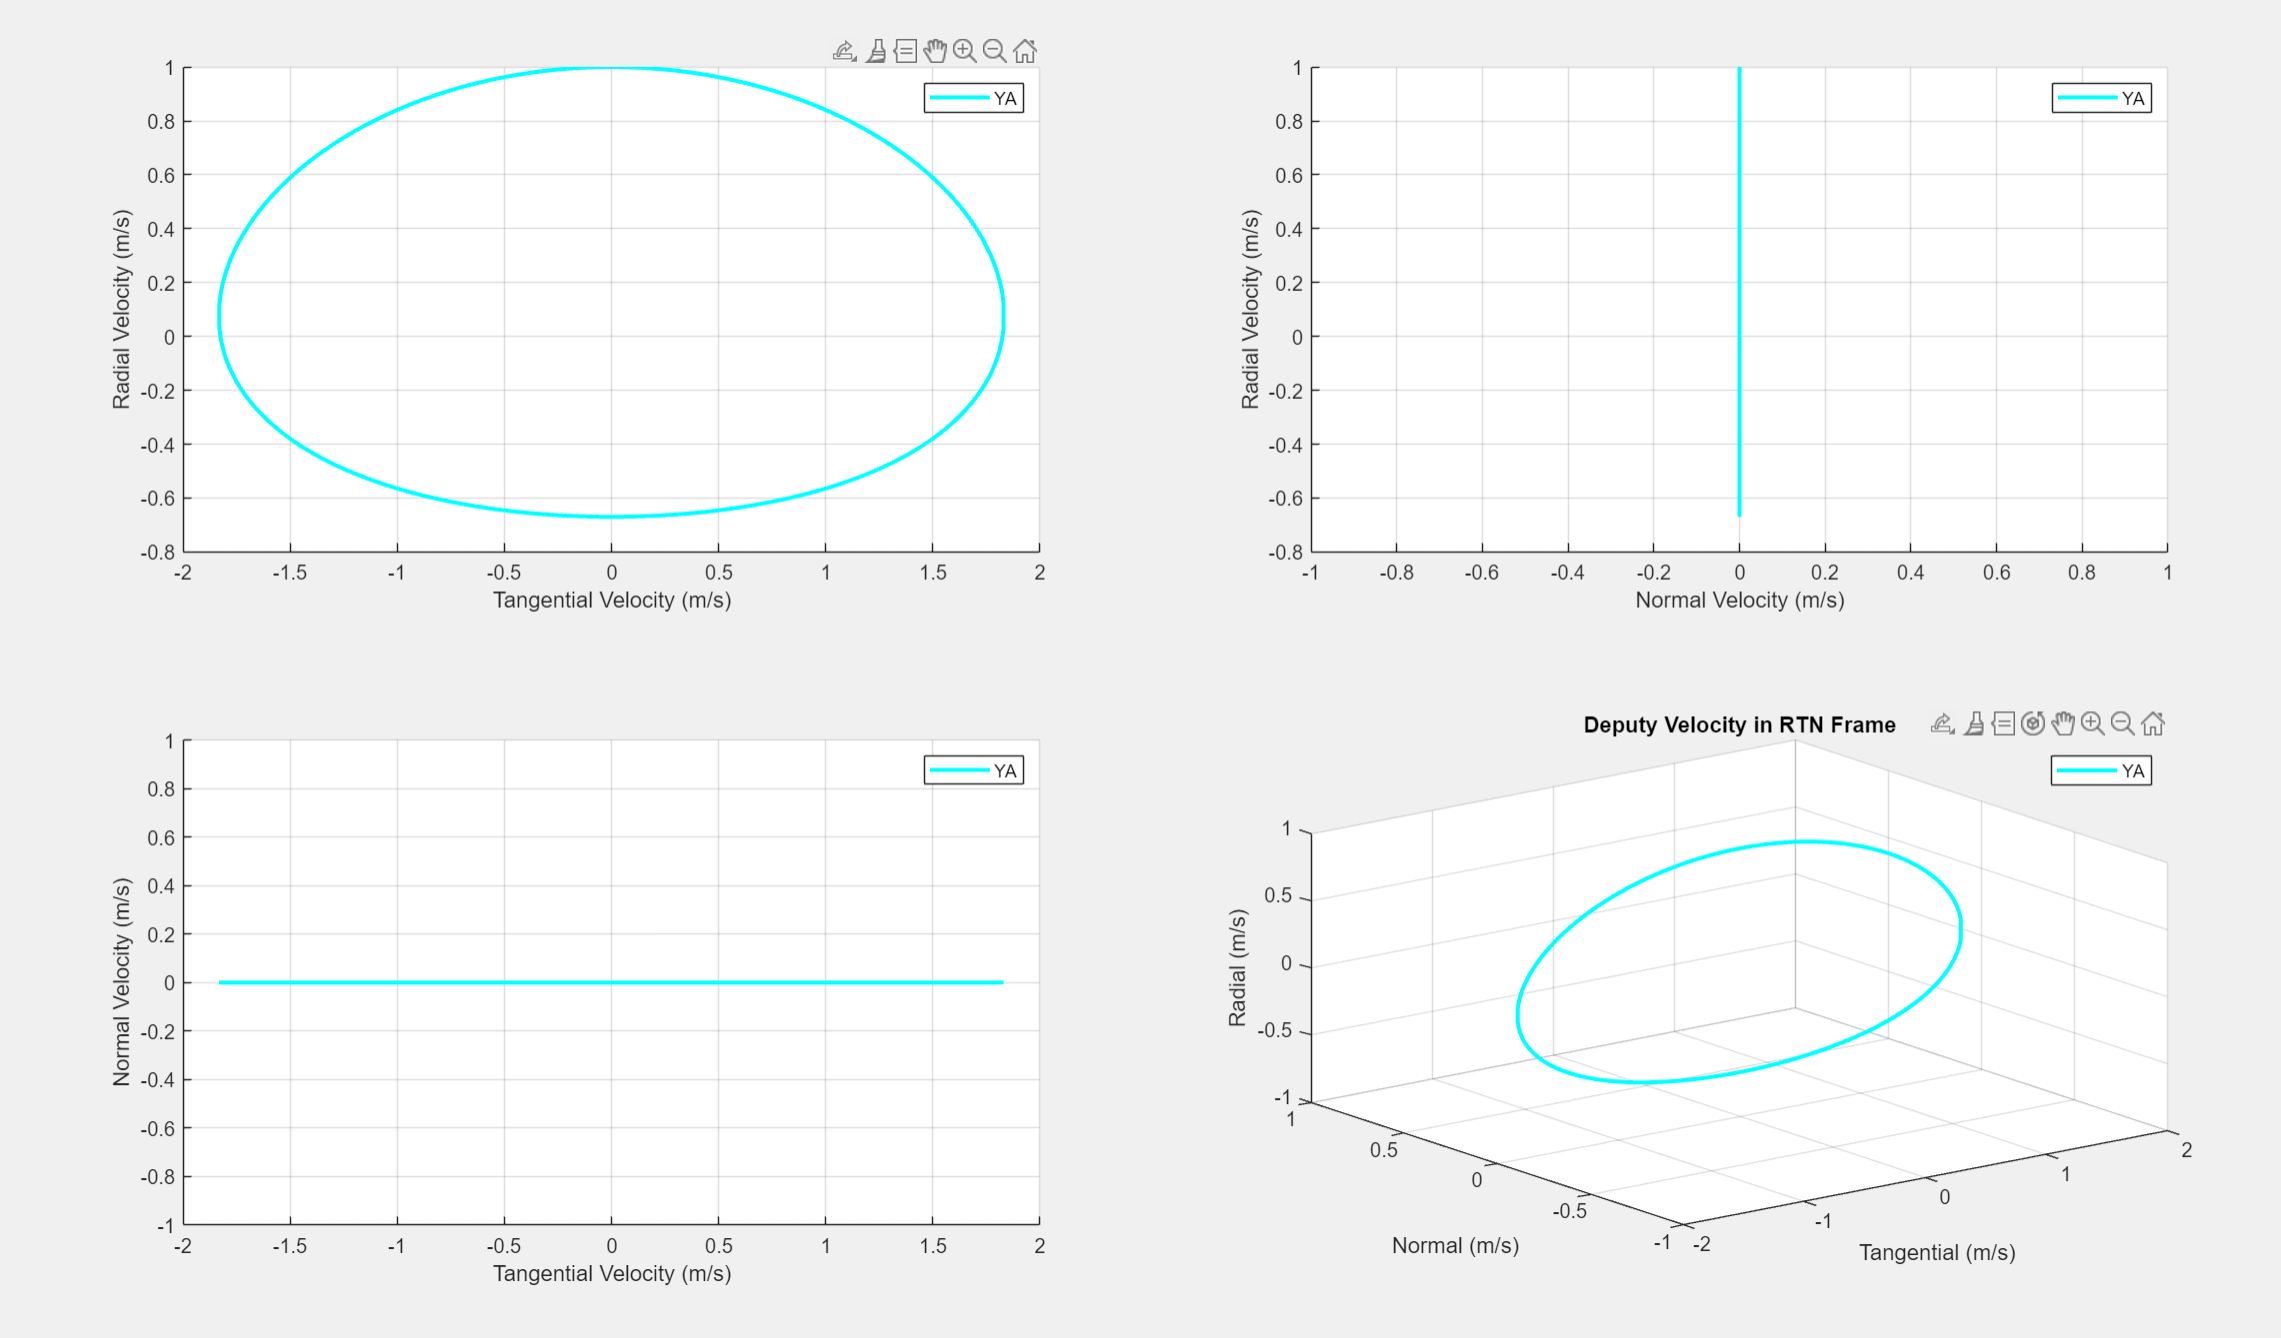
\includegraphics[width=0.7\textwidth]{PS3/Figures/YA_velocity.png}
    \caption{Deputy velocity in RTN frame from YA Equations}
    \label{fig:ya_velocity}
\end{figure}

\subsubsection{Expected Behavior}

The behavior we see in these plots aligns with expectations. Since the initial conditions involve a difference in the along track direction, with a radial velocity difference, there is no semi major axis difference, and therefore no energy difference, between the orbits. Thus, as expected, we see bounded relative motion with no drift.

\subsubsection{Propagation with ROE Geometric Mapping}
We propagate the relative motion using the geometric linear mapping with these relative orbit elements. This approach directly translates the ROE to relative position and velocity without solving differential equations.

\begin{figure}[H]
    \centering
    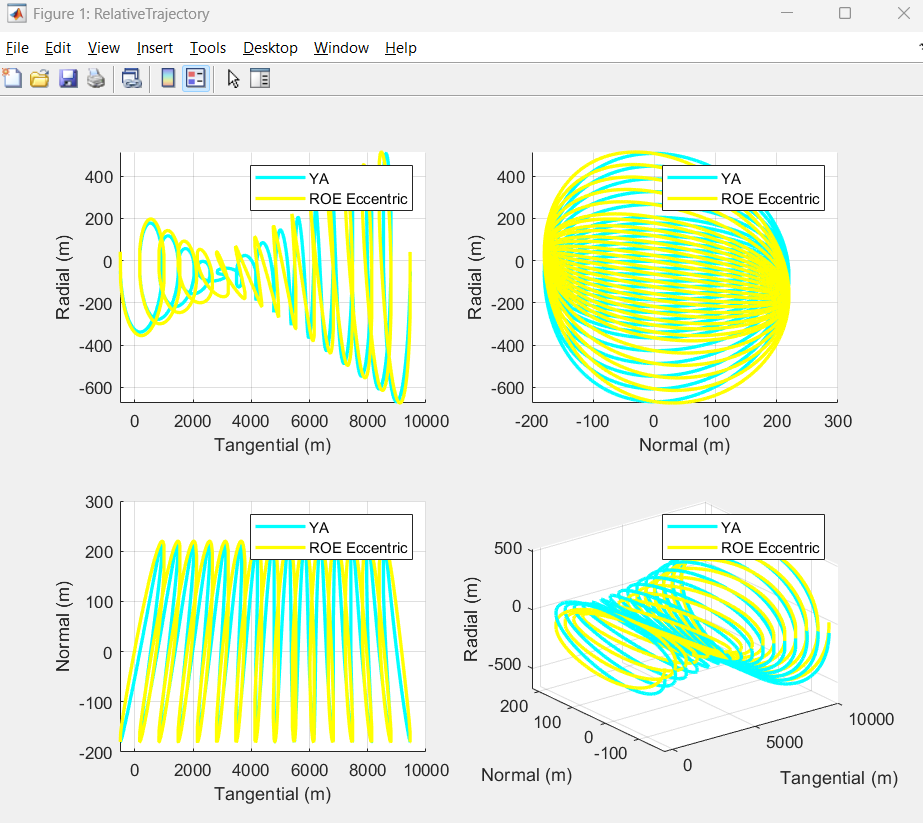
\includegraphics[width=0.7\textwidth]{PS3/Figures/ROE_YA_Position.png}
    \caption{Comparison of deputy trajectory from YA and ROE propagation in RTN frame}
    \label{fig:roe_ya_position}
\end{figure}

\begin{figure}[H]
    \centering
    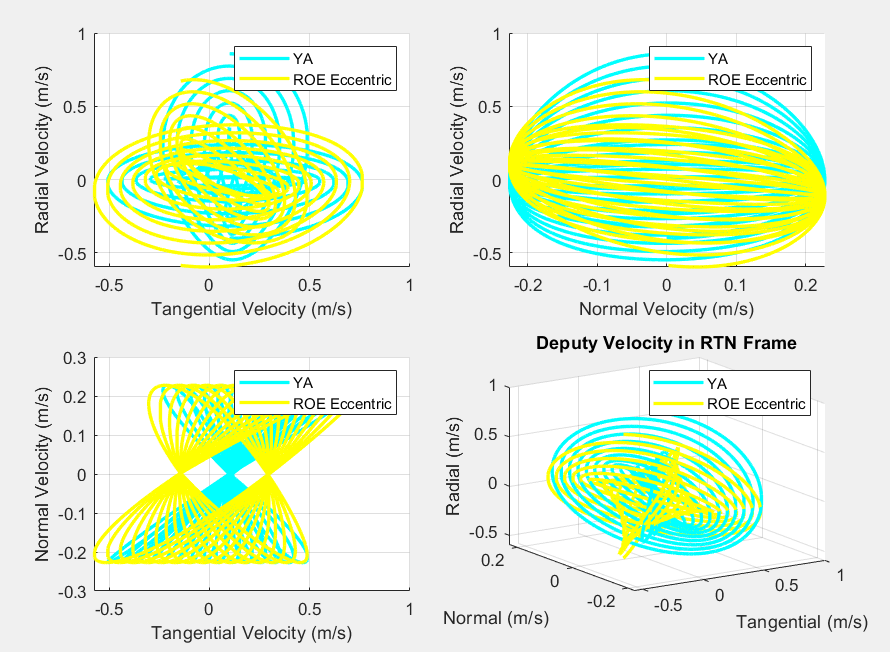
\includegraphics[width=0.7\textwidth]{PS3/Figures/ROE_YA_Velocity.png}
    \caption{Comparison of deputy velocity from YA and ROE propagation in RTN frame}
    \label{fig:roe_ya_velocity}
\end{figure}

\subsubsection{Analysis of Results}
The ROE propagation shows bounded motion as expected since δa = 0, which confirms the energy matching condition. While both YA and ROE solutions produce similar qualitative behavior, there are differences in amplitude and phase. 

The relationship between YA integration constants and ROE is mathematically consistent but not immediately obvious in the numerical values. Both represent the same physical motion using different parameterizations. The ROE approach offers a more intuitive physical interpretation, where each element corresponds directly to an aspect of relative motion.

\subsubsection{Comparison with Nonlinear Propagation}
To verify the accuracy of both solutions, we compare them with a nonlinear propagation that doesn't rely on linearization assumptions.

%\begin{figure}[H]
%    \centering
%    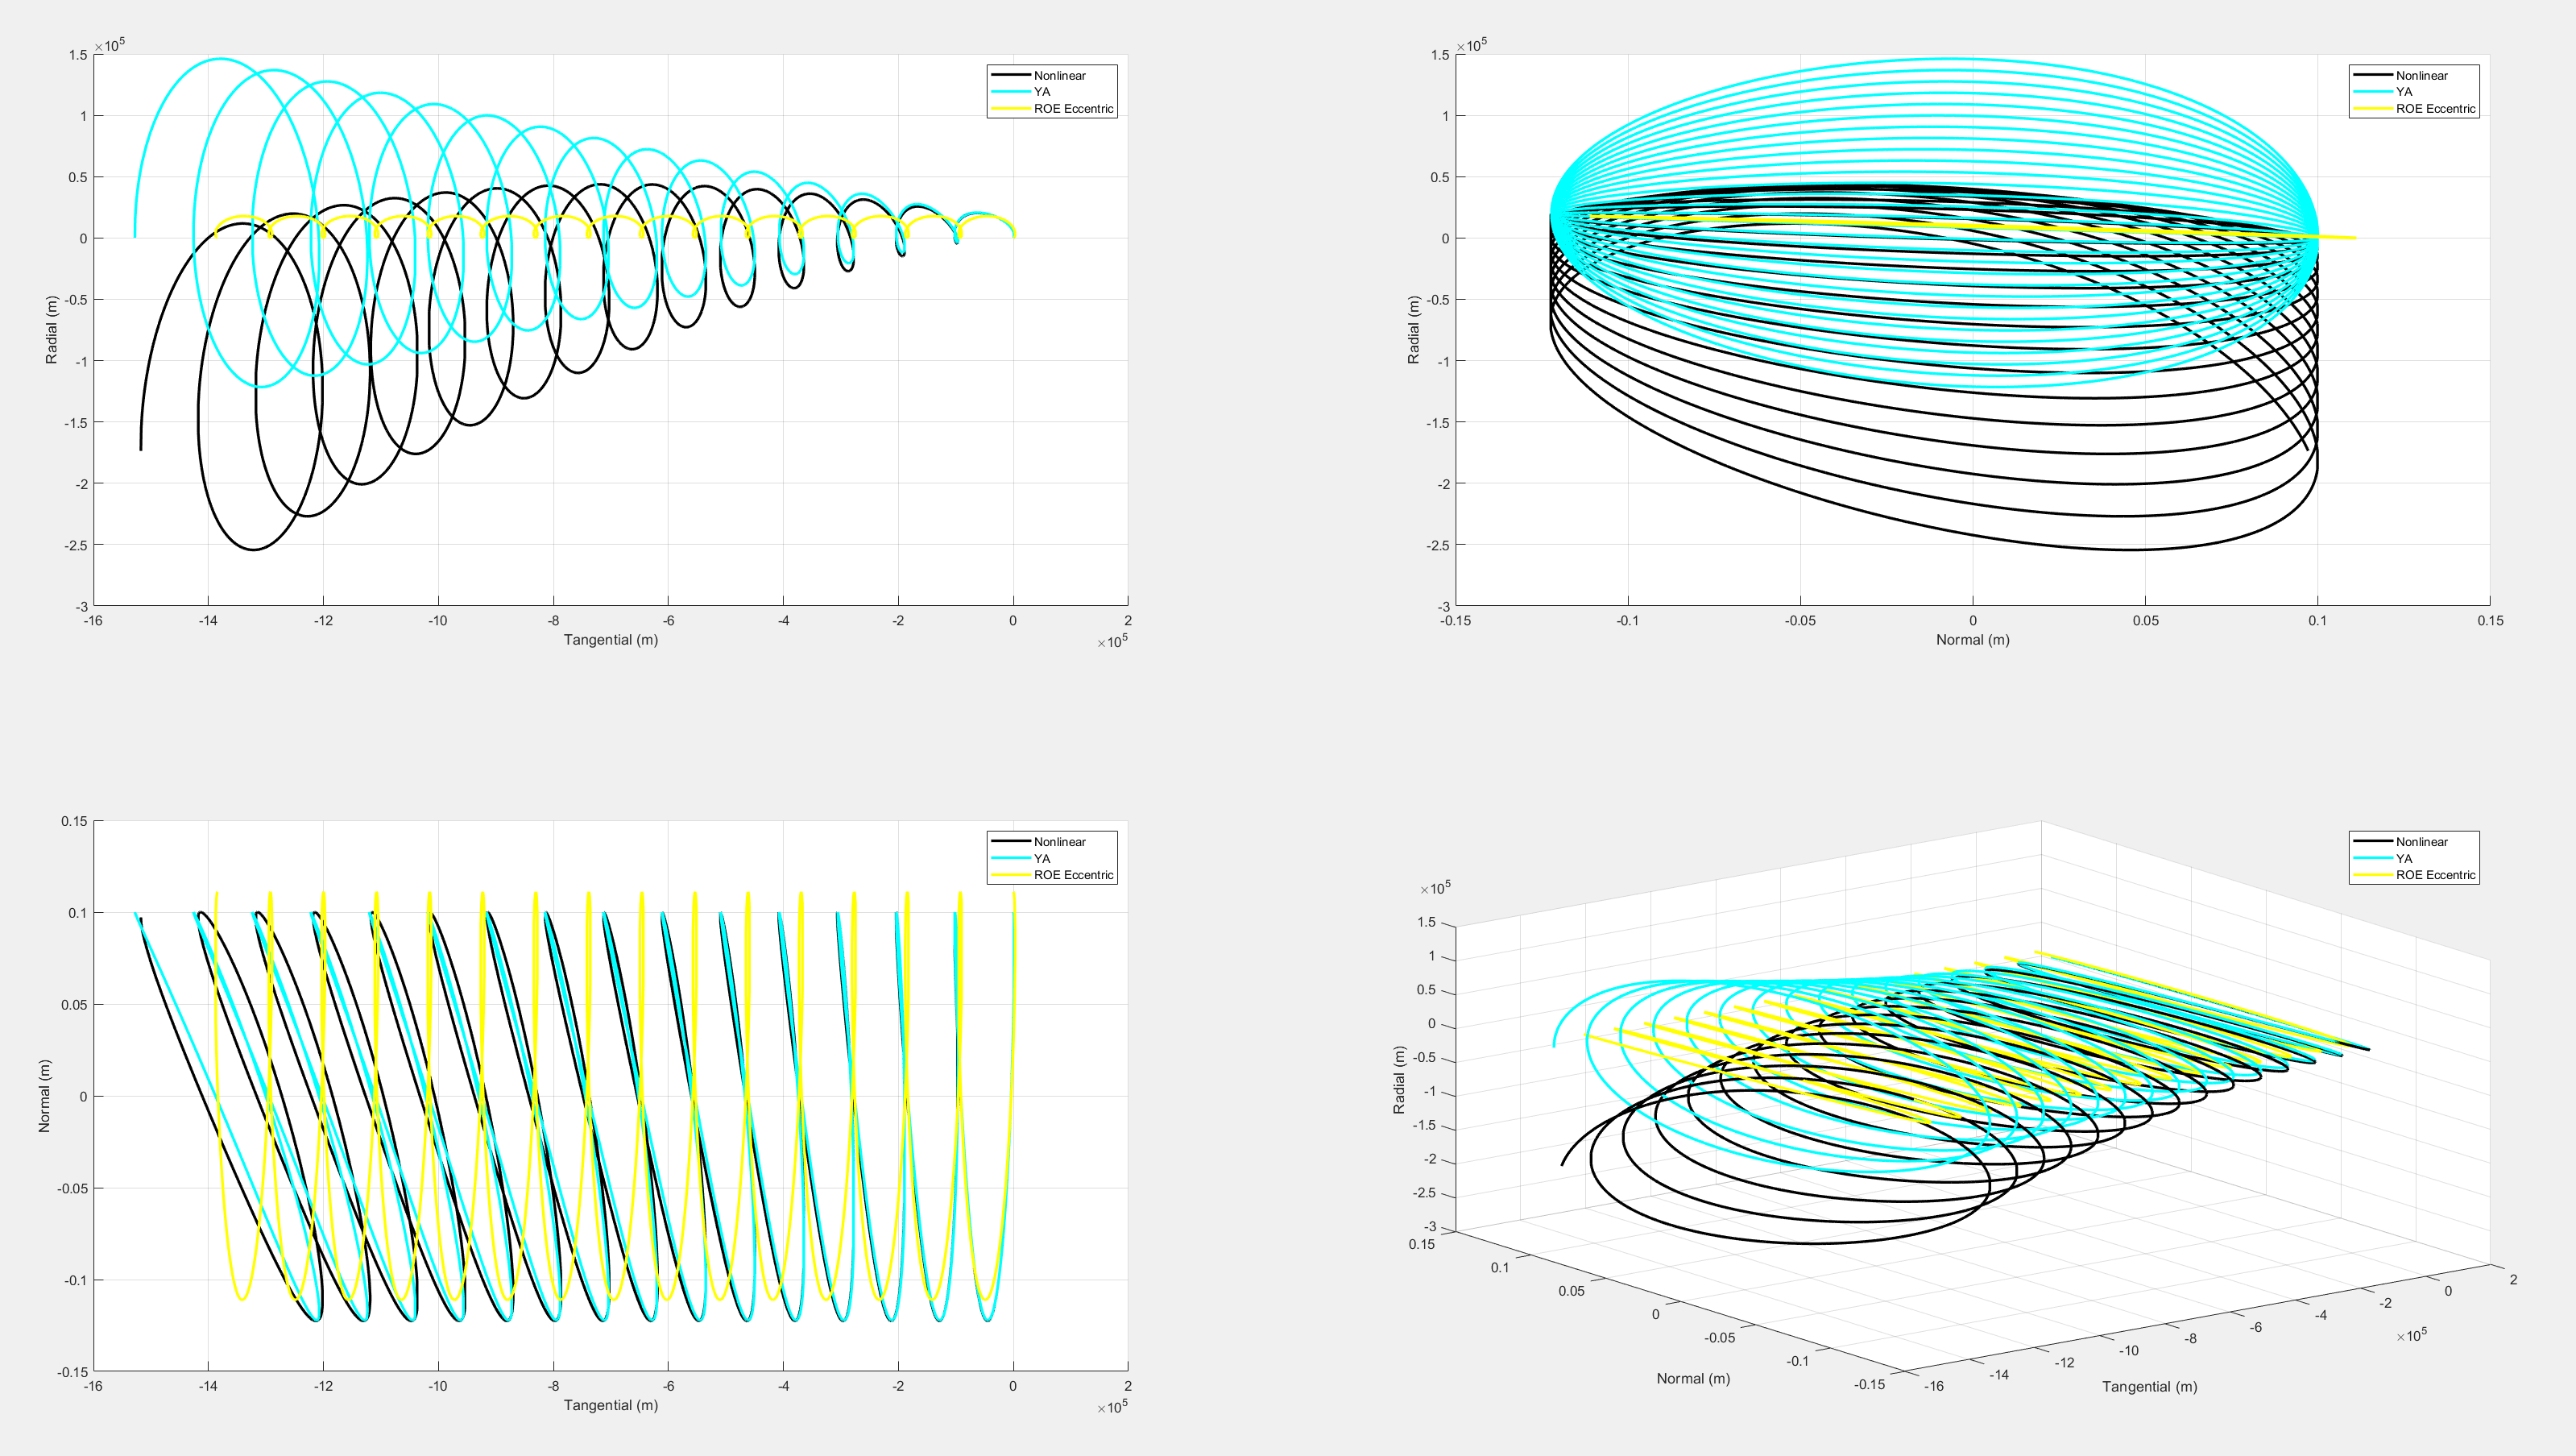
\includegraphics[width=0.7\textwidth]{PS3/Figures/Nonlinear_Position_Comparison.png}
%    \caption{Comparison of deputy trajectory with nonlinear propagation}
%    \label{fig:nonlinear_position_comparison}
%\end{figure}

%\begin{figure}[H]
%    \centering
%    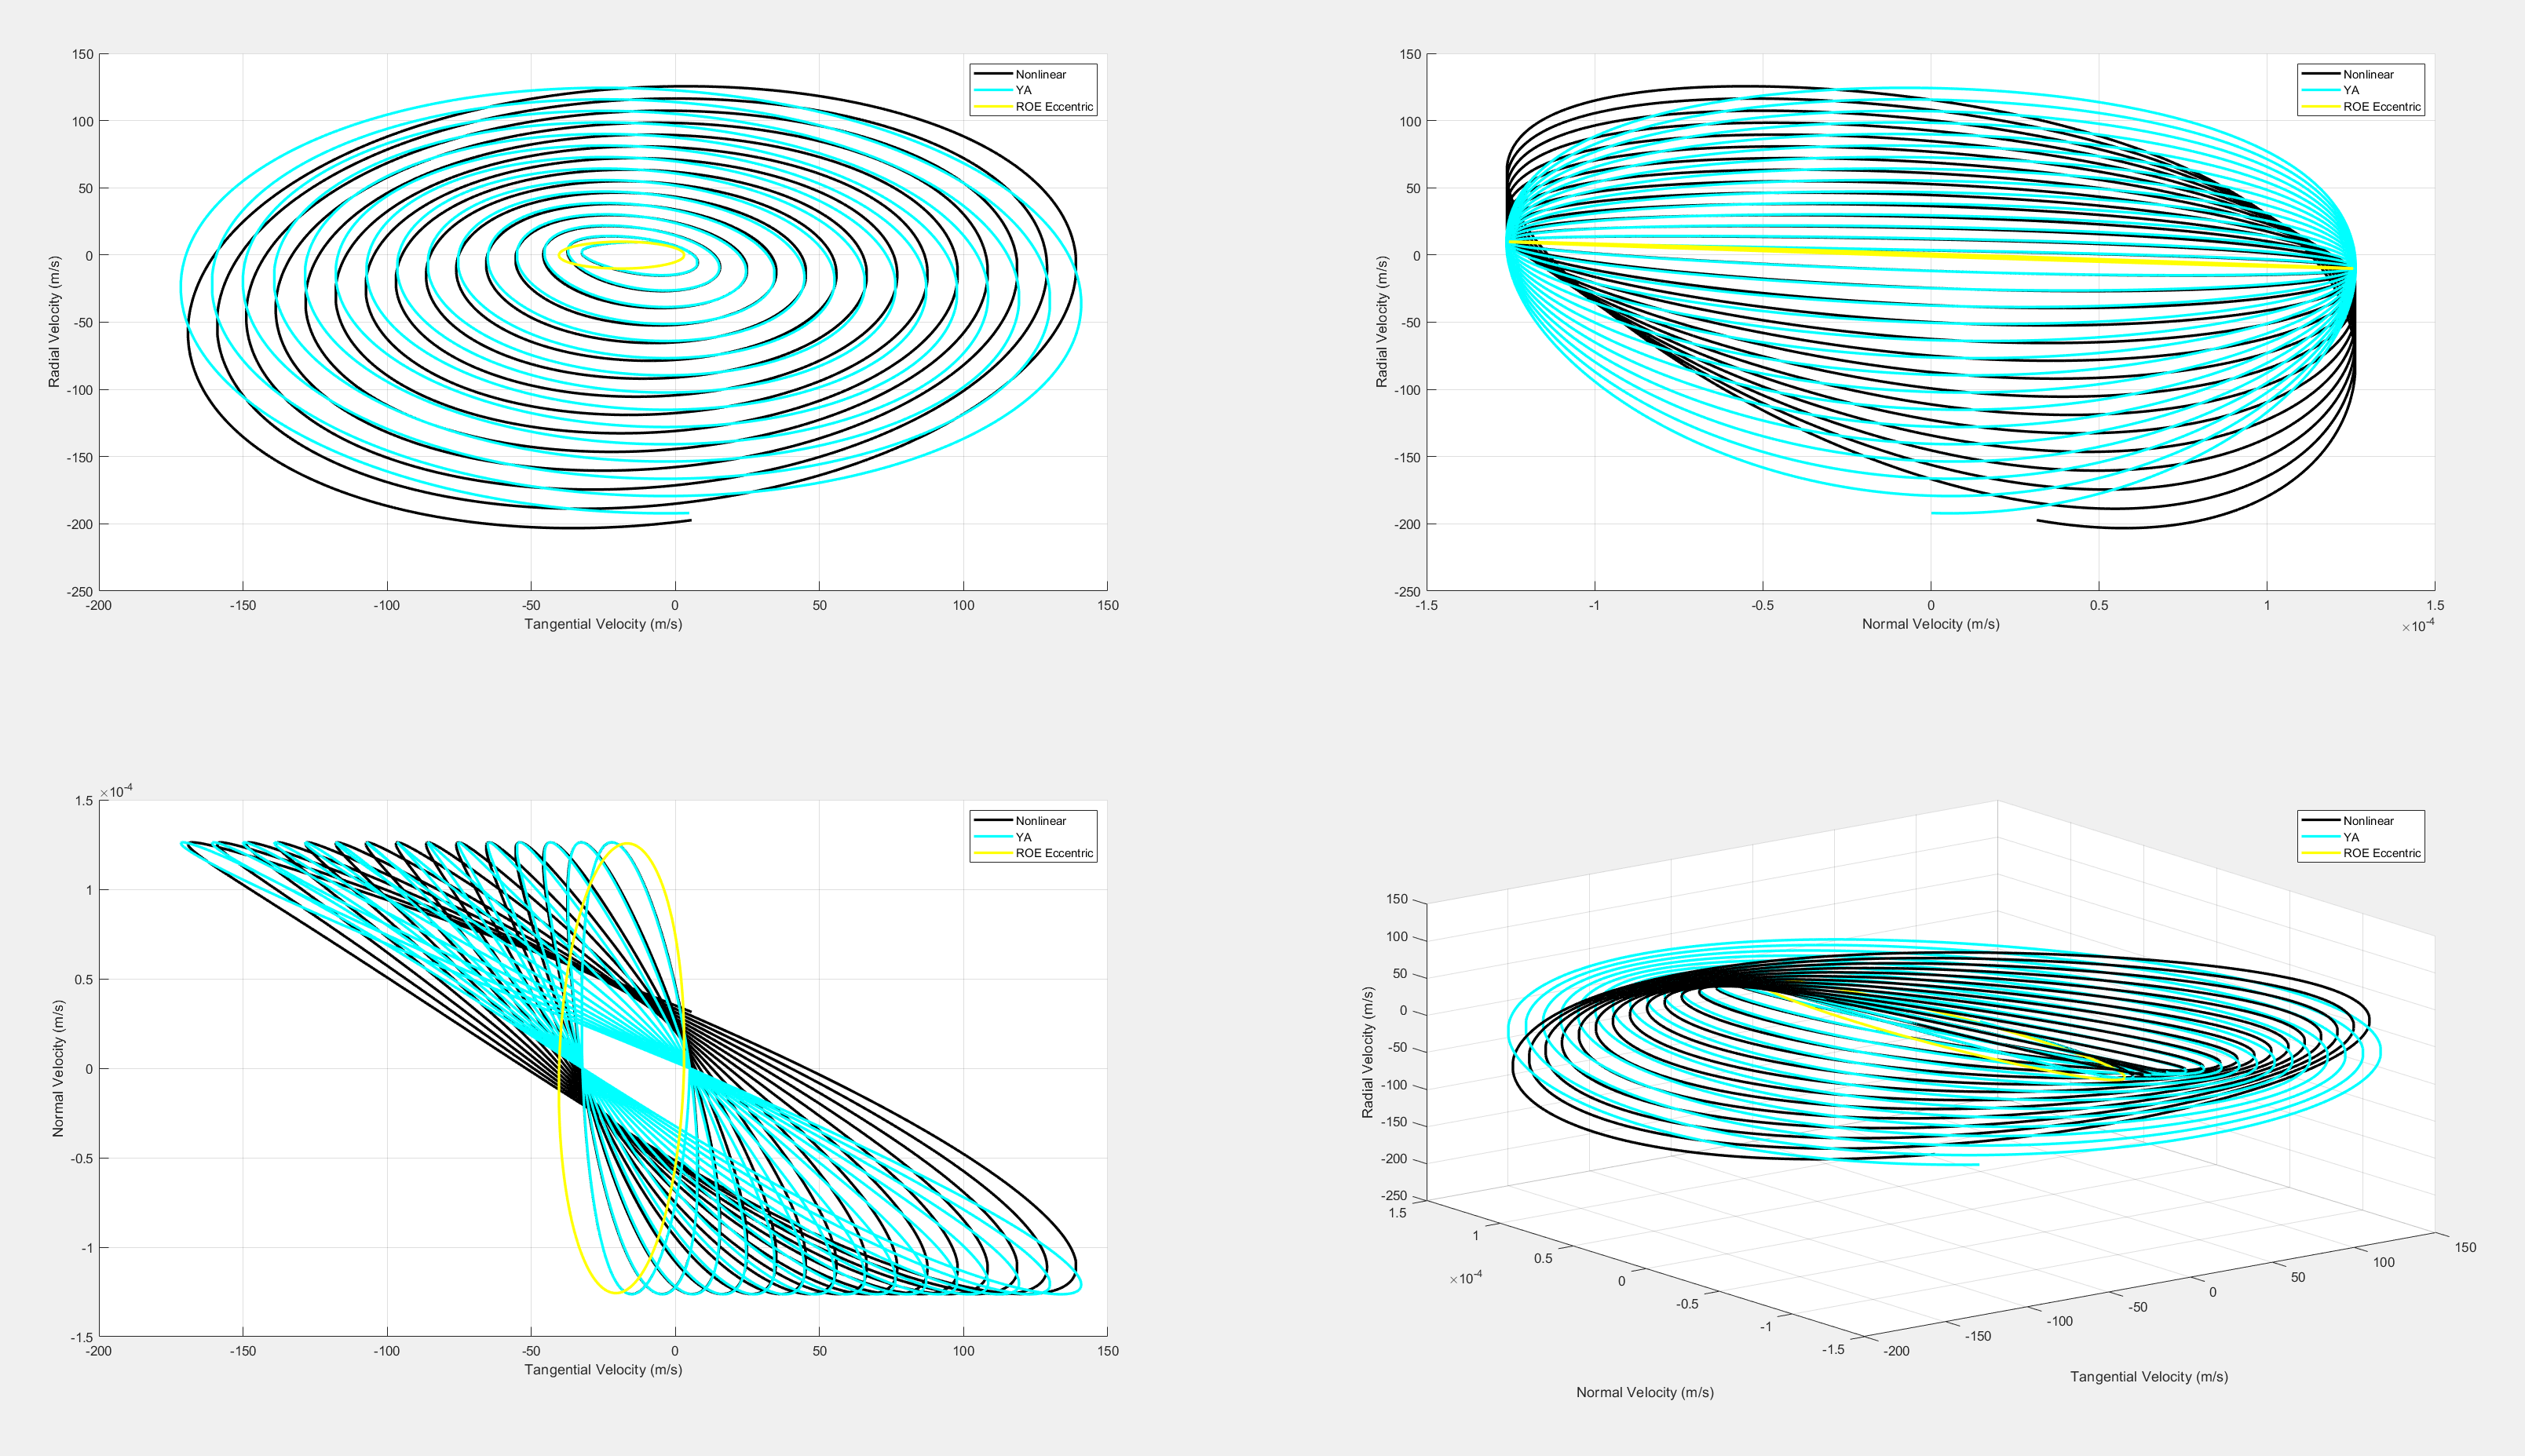
\includegraphics[width=0.7\textwidth]{PS3/Figures/Nonlinear_Velocity_Comparison.png}
%    \caption{Comparison of deputy velocity with nonlinear propagation}
%    \label{fig:nonlinear_velocity_comparison}
%\end{figure}

%\begin{figure}[H]
%    \centering
%    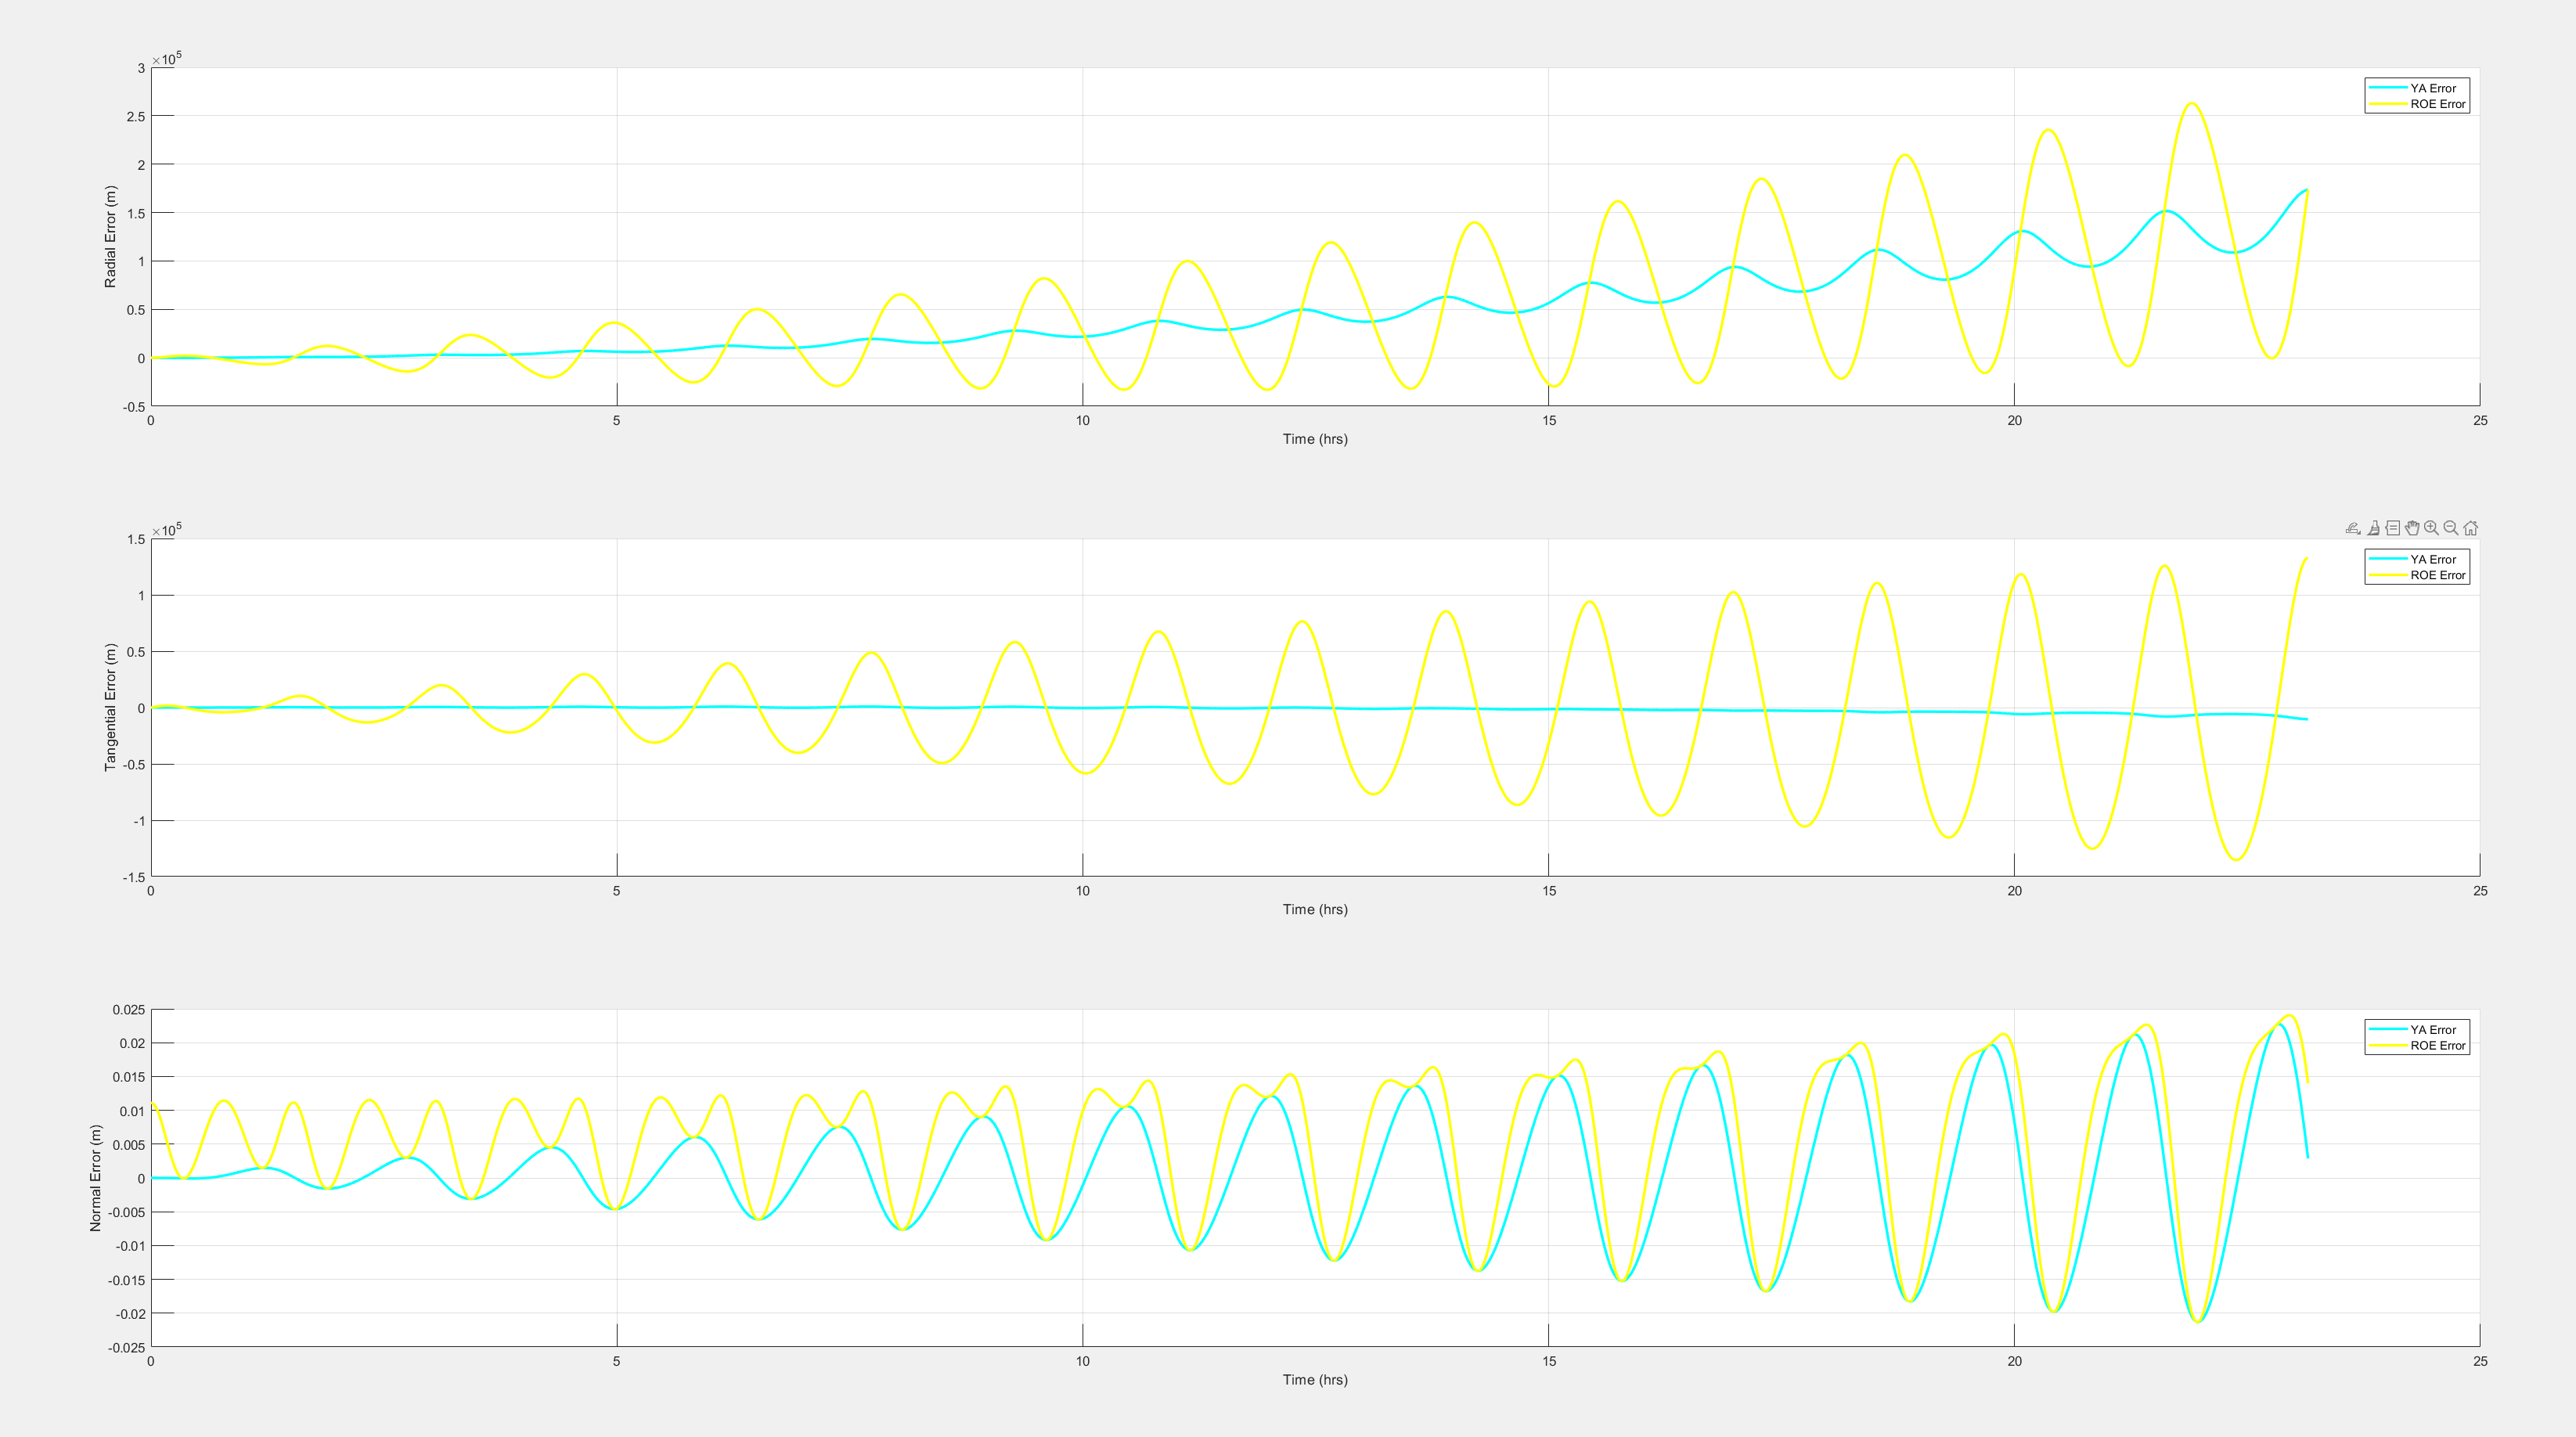
\includegraphics[width=0.7\textwidth]{PS3/Figures/Position_Error_Analysis.png}
%    \caption{Position propagation errors in RTN frame}
%    \label{fig:position_error_analysis}
%\end{figure}

%\begin{figure}[H]
%    \centering
%    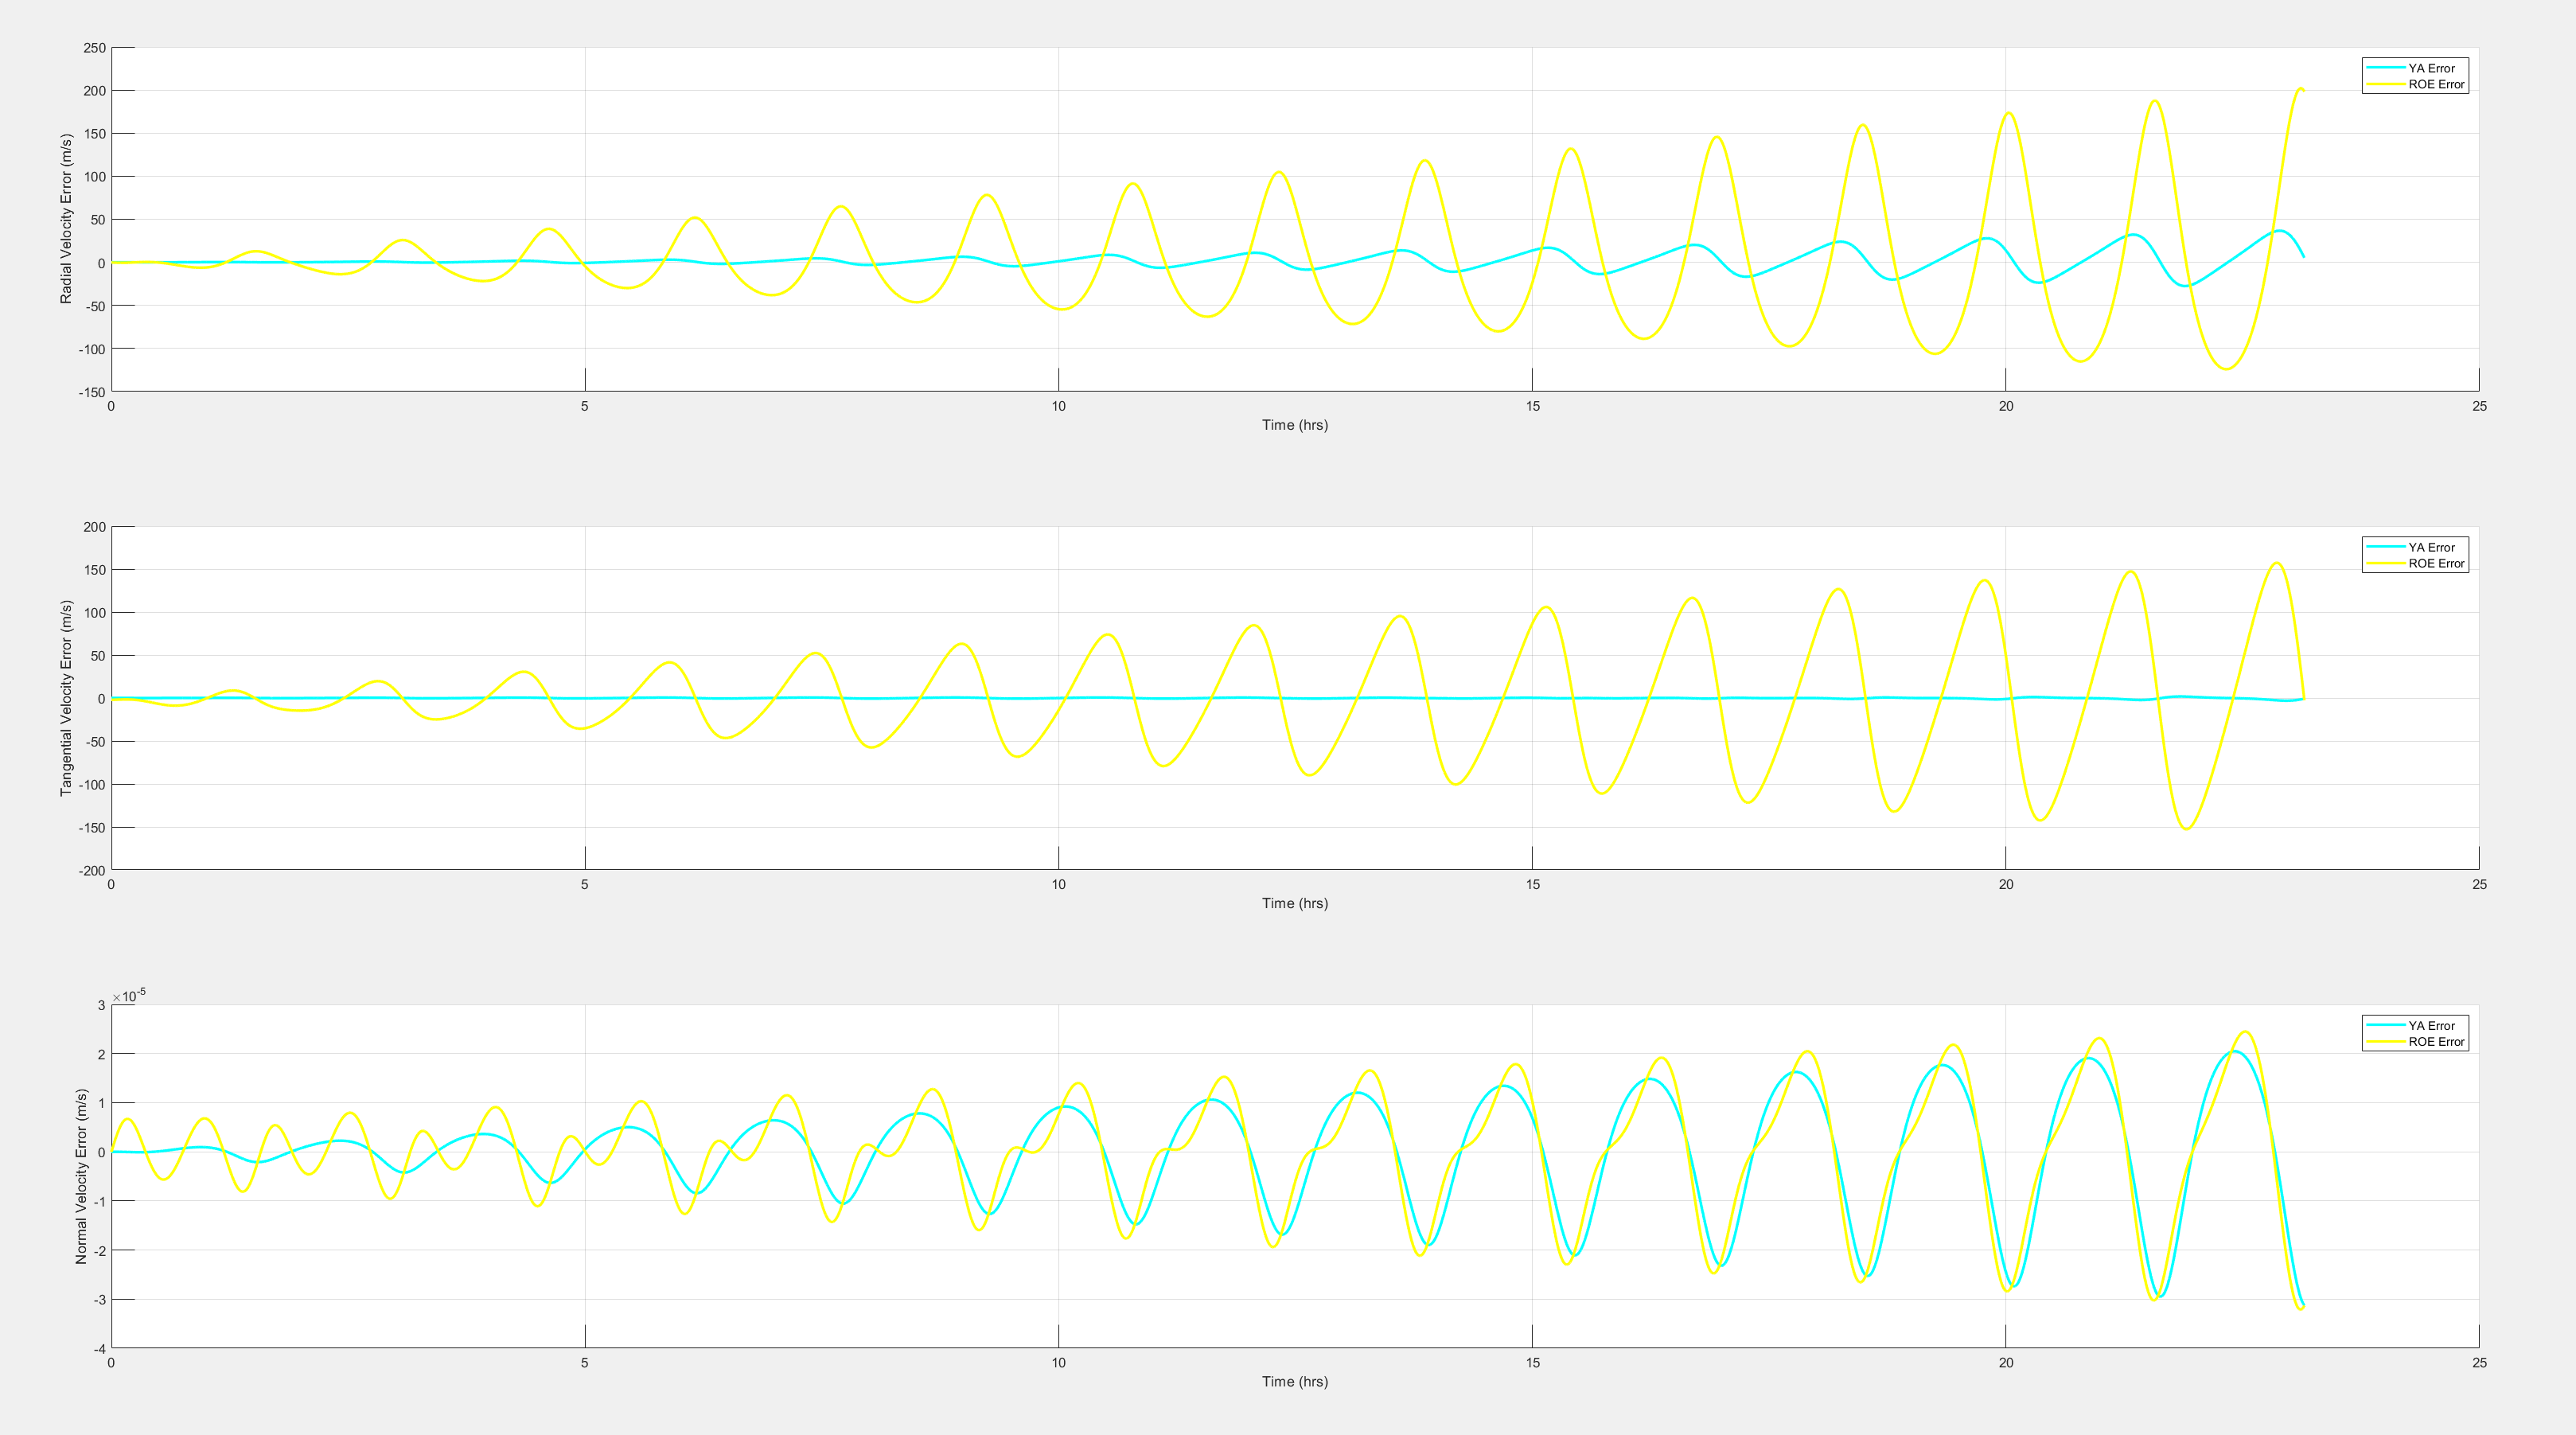
\includegraphics[width=0.7\textwidth]{PS3/Figures/Velocity_Error_Analysis.png}
%    \caption{Velocity propagation errors in RTN frame}
%    \label{fig:velocity_error_analysis}
%\end{figure}

For our scenario with e=0.1, the YA solution provides slightly better accuracy than the ROE geometric mapping implementation. The YA solution directly integrates the linearized differential equations, which can capture more dynamic effects than the static geometric mapping used in our ROE implementation. However, both methods show good qualitative agreement with the nonlinear solution.

\subsubsection{Case Study: Semi-Major Axis Difference}
We now modify our initial conditions to include a radial offset of 10 meters, creating a small difference in semi-major axis. This value is small enough to remain within linearization assumptions but large enough to produce visible drift over 15 orbits.

%\begin{figure}[H]
%    \centering
%    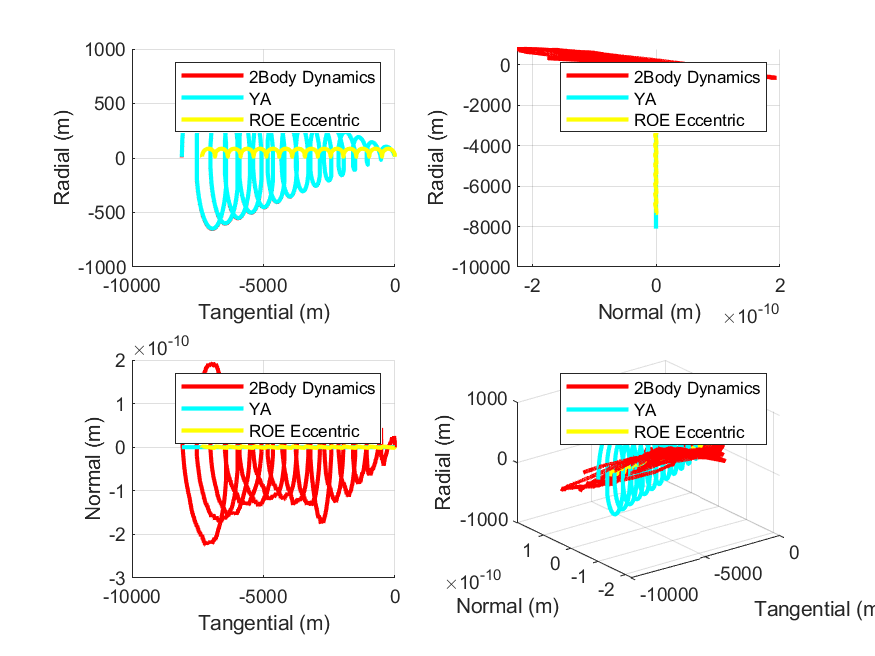
\includegraphics[width=0.7\textwidth]{PS3/Figures/SMA_Difference_Position.png}
%    \caption{Deputy trajectory with semi-major axis difference}
%    \label{fig:sma_difference_position}
%\end{figure}

%\begin{figure}[H]
%    \centering
%    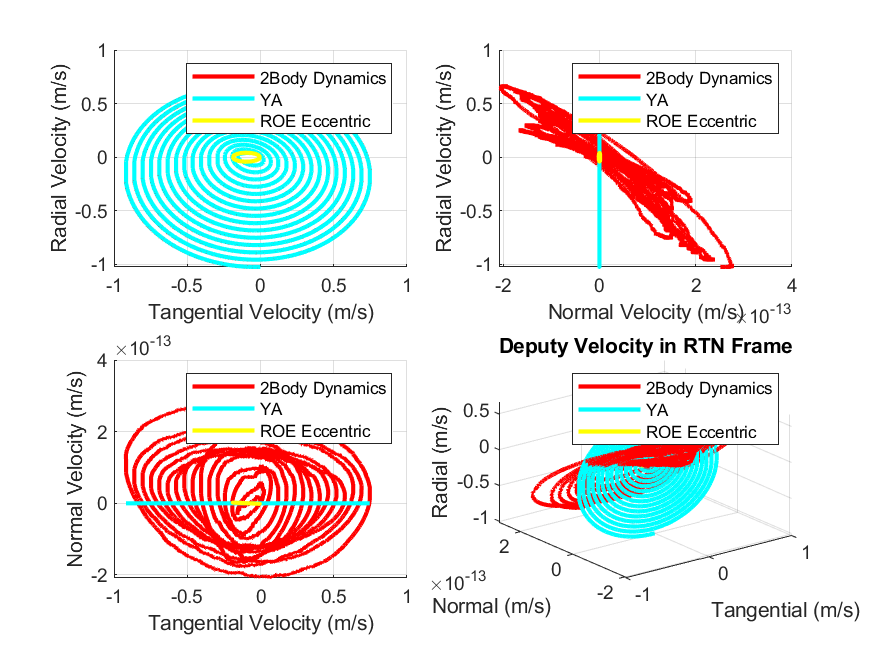
\includegraphics[width=0.7\textwidth]{PS3/Figures/SMA_Difference_Velocity.png}
%    \caption{Deputy velocity with semi-major axis difference}
%    \label{fig:sma_difference_velocity}
%\end{figure}

As expected, the results show secular drift in the along-track direction due to the different orbital periods. Both analytical solutions correctly capture this drift, which increases approximately linearly with time. The drift rate matches the theoretical prediction.

\subsubsection{Case Study: Highly Eccentric Orbit}
Finally, we analyze a case with high eccentricity (e=0.6) to test the limits of our linearized models.

%\begin{figure}[H]
%    \centering
%    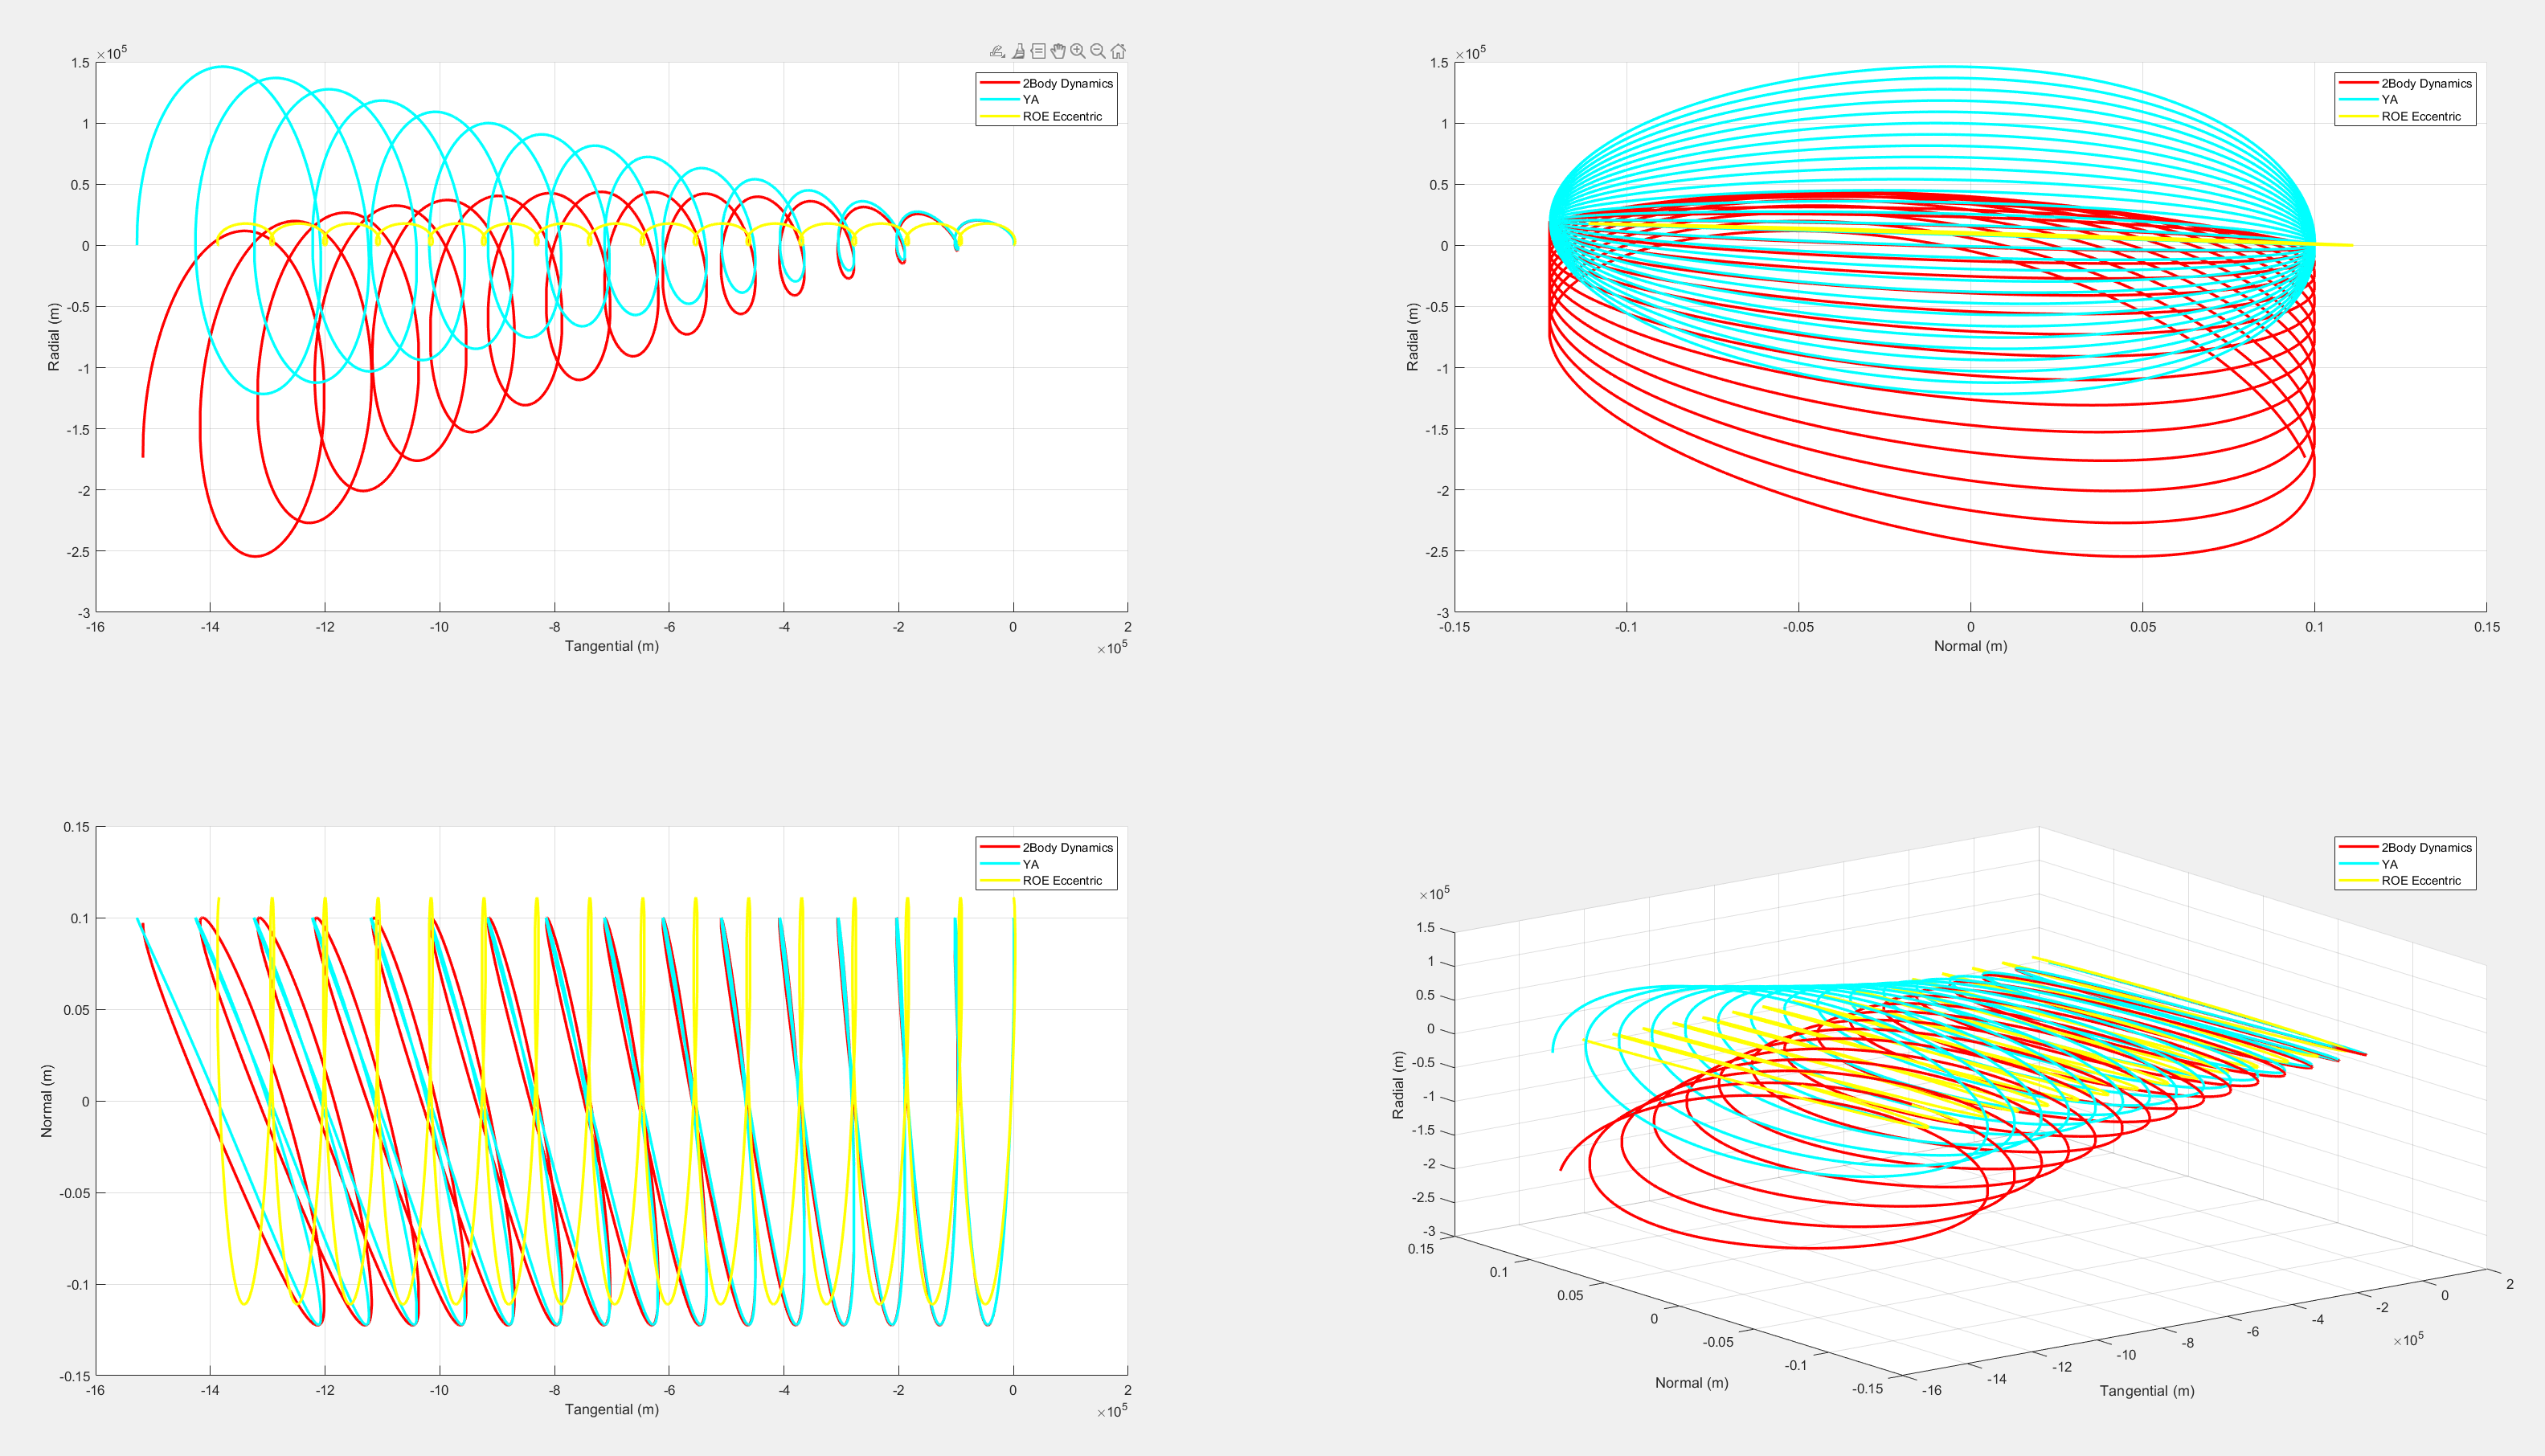
\includegraphics[width=0.7\textwidth]{PS3/Figures/High_Eccentricity_Position.png}
%    \caption{Deputy trajectory with highly eccentric orbit (e=0.6)}
%    \label{fig:high_eccentricity_position}
%\end{figure}

%\begin{figure}[H]
%    \centering
%    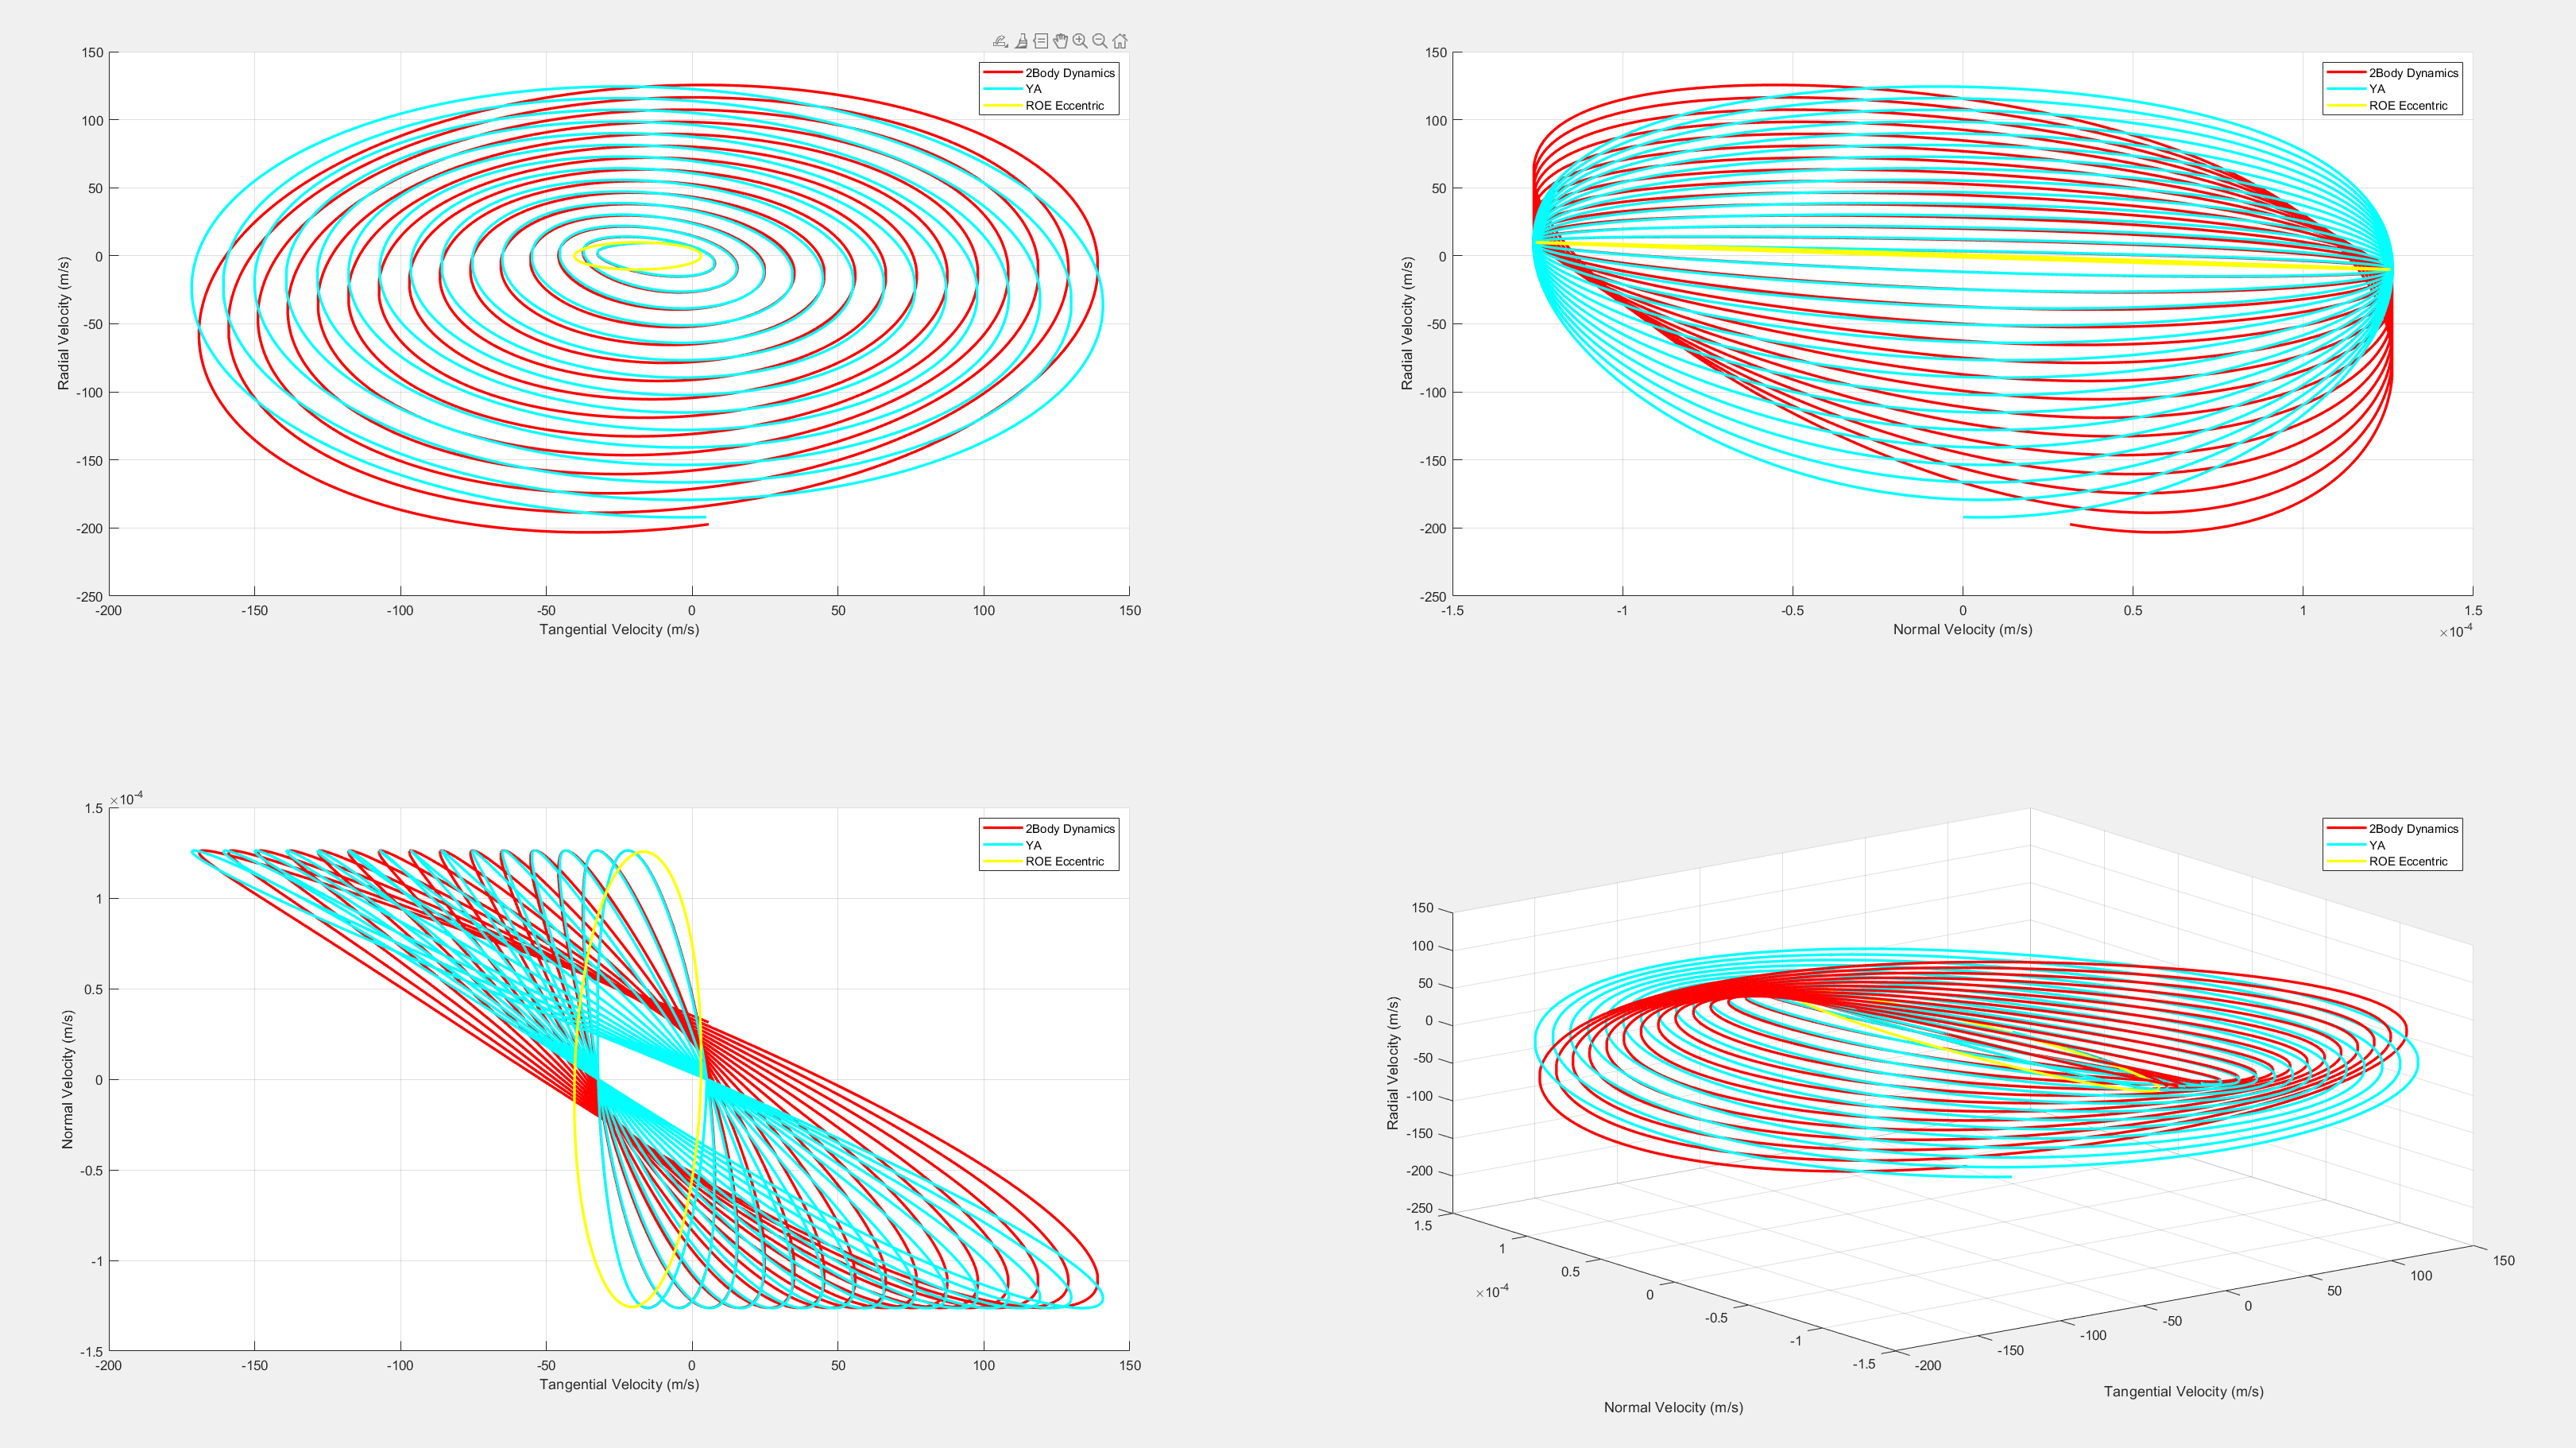
\includegraphics[width=0.7\textwidth]{PS3/Figures/High_Eccentricity_Velocity.png}
%    \caption{Deputy velocity with highly eccentric orbit (e=0.6)}
%    \label{fig:high_eccentricity_velocity}
%\end{figure}

At this high eccentricity, we observe significant deviations between the linearized solutions and the nonlinear truth. The relative motion shows strong distortions near perigee passages, where orbital velocity changes rapidly. This demonstrates the limitations of linearized theories for highly eccentric orbits, as the linearization assumptions break down when eccentricity increases. For such cases, higher-order models or fully nonlinear methods would be required for accurate prediction of relative motion.